% !TeX root = ../车云协同液罐车防侧翻行驶规划与控制研究.tex

\chapter{引言}
\label{chap:introduction}

\section{研究背景及意义}
\label{sec:background_and_significance}

  我国危化品运输需求持续增长，2025年危化品运输总额已接近3万亿元，其中利用液罐车通过公路运输的超过\SI{80}{\percent}\cite{qianyuyan2023}，液罐车在危化品公路运输中占据重要地位。据统计，截至2025年，我国危化品运输车辆总数超过36万辆，其中液罐车数量接近19万辆，占比高达\SI{52.8}{\percent}\cite{zhongguowuliulianhehui2022}。然而，液罐车在运输过程中存在较高的安全风险。2011年至2025年间，我国共发生超过1万5千起危化品罐车运输重大事故，其中\SI{78.7}{\percent}的事故发生在液罐车行驶过程中，\SI{62.7}{\percent}的事故是由车辆侧翻引起\cite{liuhuipling2023, chengshuo2023, lijian2014,chenxiaoyong2023, wangyang2023}。液罐车侧翻事故在货车严重伤亡事故中占比超过\SI{31}{\percent}，液罐车单方面事故中侧翻占比接近\SI{70}{\percent}\cite{authority_tank_truck2022}，可见液罐车侧倾稳定性差易于侧翻的特性。

  频发的液罐车侧翻事故后果严重。如图~\ref{fig:severe_results}所示，2020年6月13日，浙江温岭G15高速，一辆满载25.36吨液化石油气的液罐车因超速侧翻爆炸，导致20人死亡，175人受伤，数十间房屋倒塌，200余间成危楼\cite{wenling_accident2022}；2022年四川江油县，一辆液罐车因超速失控侧翻造成8死20伤；2022年山东威海，一辆液罐车路口躲避变道车辆侧翻致多人遇难；2023年广西百色，液罐车在高架桥转弯时因车速过快侧翻爆炸多人遇难；2023年北京东六环，液罐车避让施工侧翻爆炸致多人死亡；2023年湖南邵阳，液罐车下坡急转向时因车速过快侧翻40顿柴油泄漏……因侧翻车辆装载液化石油/天然气、汽柴油、甲醇等易燃易爆品的情况占\SI{86}{\percent}以上\cite{qianyuyan2023}，因此事故常伴随危化品液体泄漏，常造成环境污染、燃烧、爆炸等严重次生灾害，酿成重大人员伤亡和财产损失\cite{liuhuipling2023, chengshuo2023, lijian2014,chenxiaoyong2023, wangyang2023,authority_tank_truck2022,wenling_accident2022, baijinghua2023}。故解决液罐车运输过程中的侧翻问题迫在眉睫。


  \begin{figure}
    \centering
    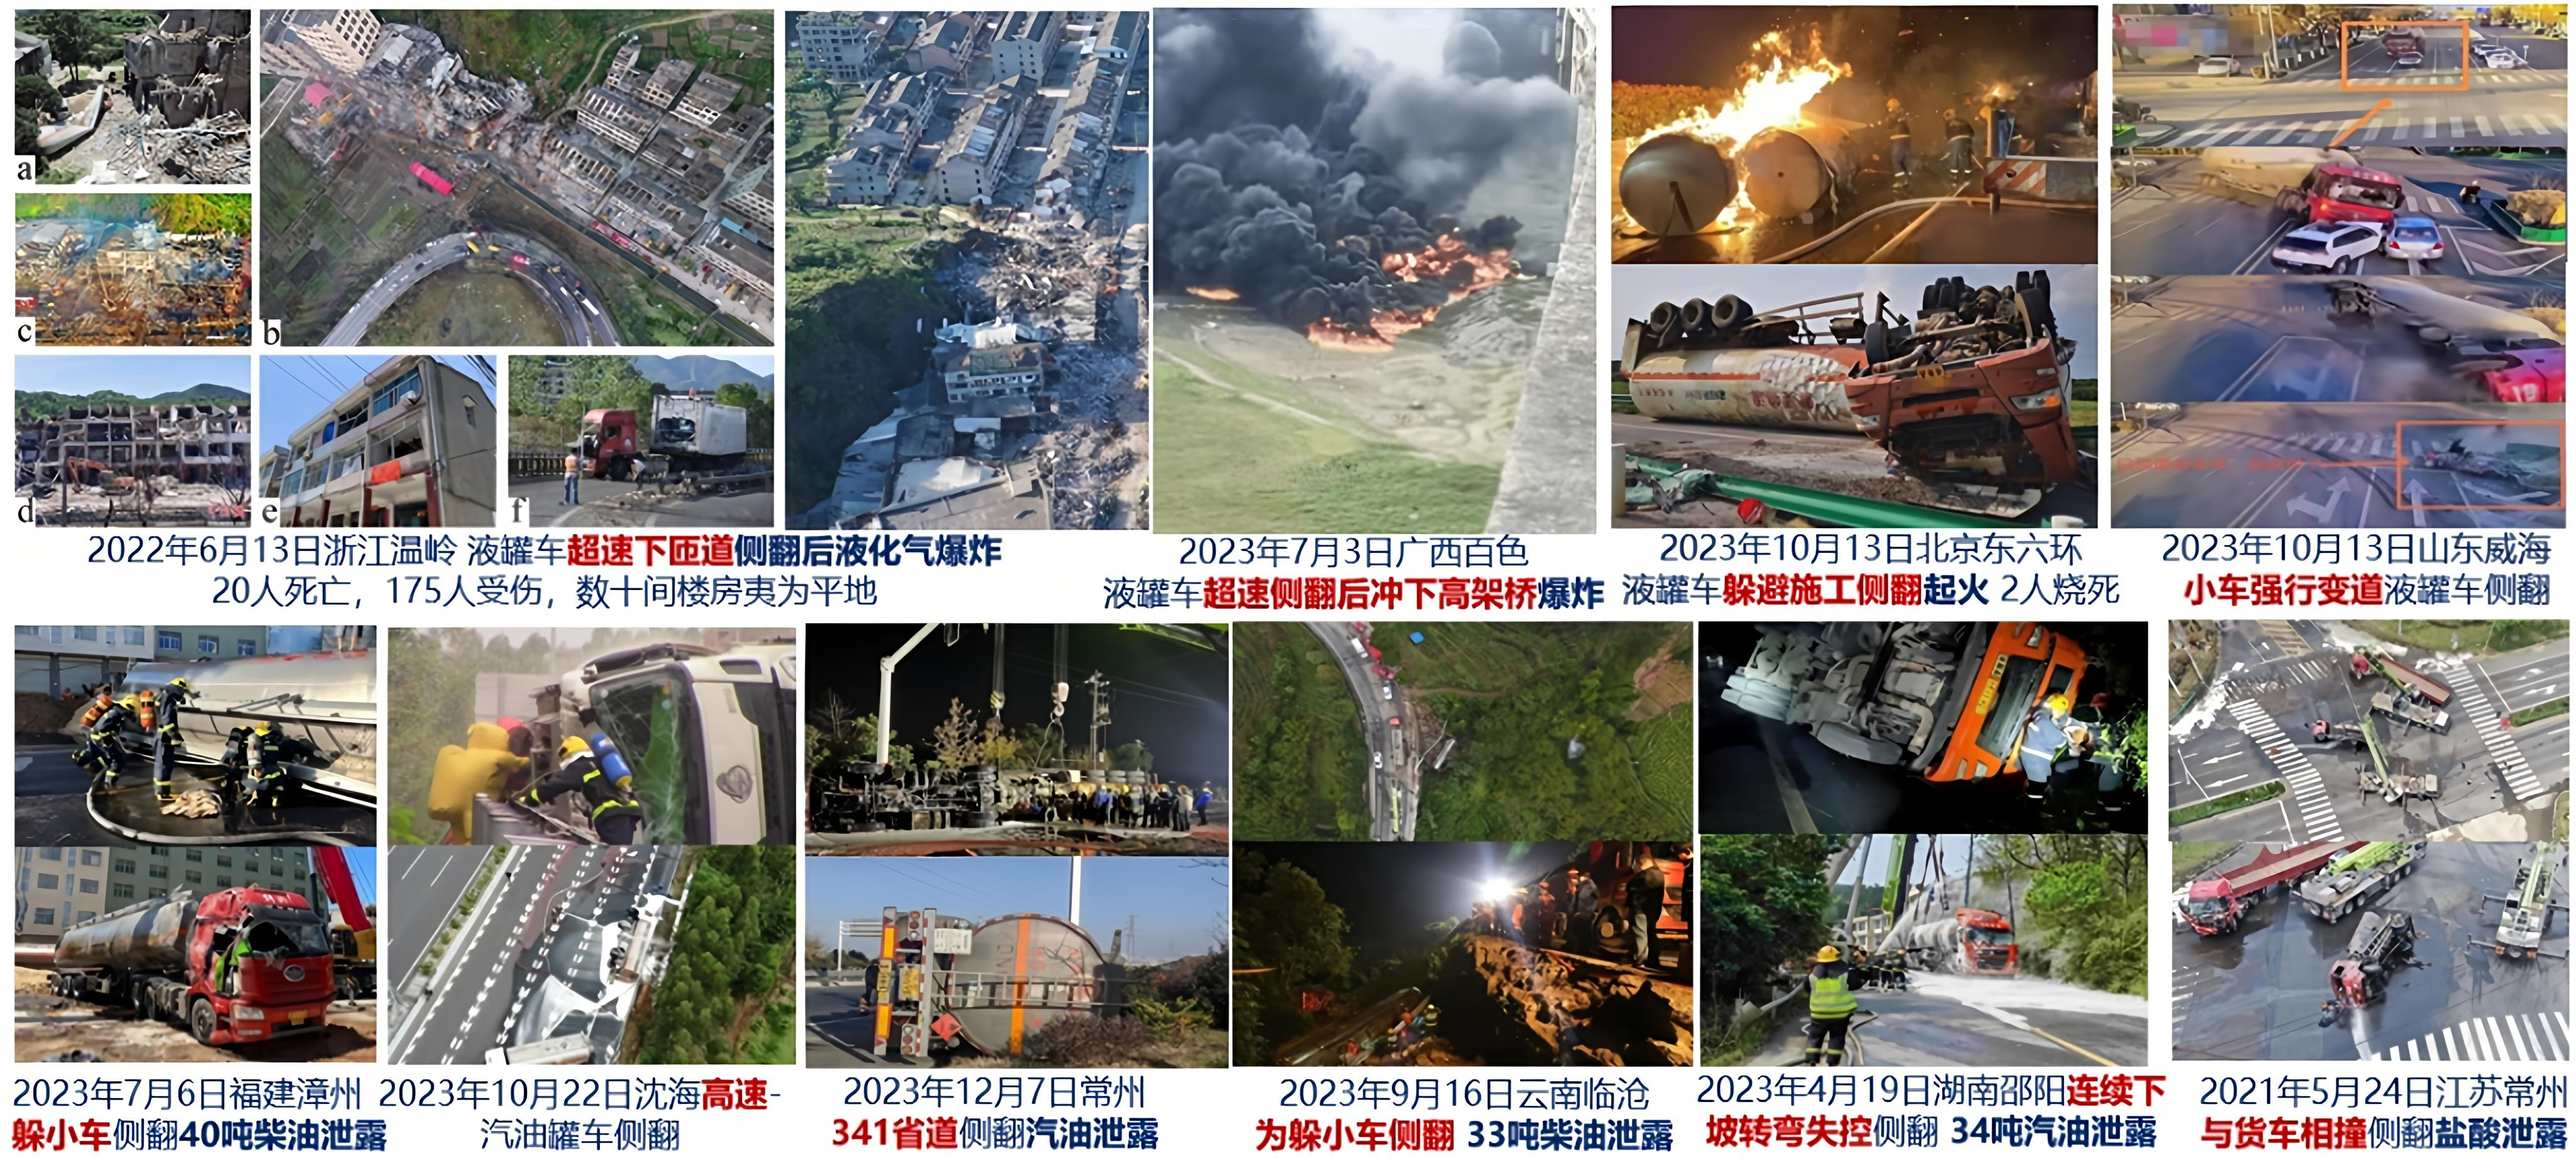
\includegraphics[width=0.9\linewidth]{fig/chap1/severe_results.jpg}
    % \caption*{图片注释解释说明}
    \caption{液罐车事故及其严重后果}
    \label{fig:severe_results}
  \end{figure} 

  液罐车侧翻事故原因可归结为三方面：非满载车液耦合侧向稳定性差的车辆特性，驾驶员对动静态交通信息（道路结构、临时施工、周车状态与意图等）掌握不足的单车局限，以及超速、疲劳驾驶等违法行为及救车失误的人因失误。

  （1）\emph{车辆特性}：液罐车因车辆液体耦合的非满载状态下侧向稳定性差，易发生侧翻。根据现行标准，液罐车必须非满载运行，以避免液体膨胀、蒸汽压力升高引发的泄漏或爆炸，最大允许充液量不得超过\SI{95}{\percent}\cite{biaozhun185642006,biaozhunR00052011}。液罐车在卸货途中通常保持中低充液率，这会导致液体晃动，明显降低车辆的侧倾稳定性。

  （2）\emph{单车局限}：驾驶员对动静态交通信息的掌握不足，是正常路段事故的主要原因，主要受限于以单车视角对周围环境、车辆状态和意图的感知能力\cite{authority_tank_truck2022}。特殊路段以及他车危险动态使得驾驶员需及时响应，大曲率弯道和坡道等将改变液体晃动与车辆的侧倾特性若不注意易引起事故。

  （3）\emph{人因失误}：超速、疲劳驾驶等违法行为，以及紧急工况下由于驾驶员不够熟练而造成的救车失误等由于人因造成的本可以避免的因素而加剧了危险情况下的侧翻风险。

  上述人因、单车局限及车辆特性驱动的侧翻风险，促使自动驾驶技术成为解决液罐车安全问题的潜在路径。自动驾驶可消除超速、疲劳驾驶等违法行为，通过多传感器融合实现360°无盲区感知，缓解人类感知盲区，其优化控制算法能更快速准确地响应动态环境，避免紧急工况下的救车失误。

  \begin{figure}
      \centering
      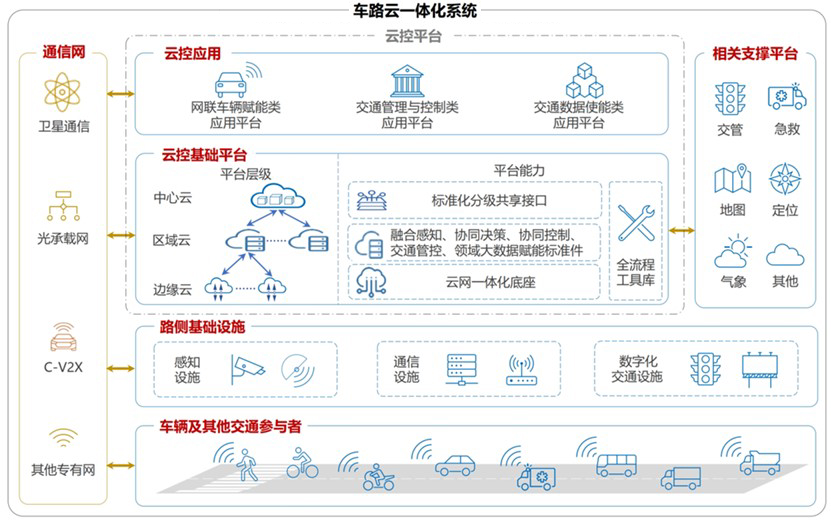
\includegraphics[width=0.9\linewidth]{fig/chap1/cloud_platform.jpg}
      \caption{车路云一体化系统架构\cite{icv2023whiteroadcloud}} 
      \label{fig:cloud_platform}
  \end{figure}

  近年来，商用车自动驾驶技术取得显著成果。2024年卡尔动力2-6车混合无人化半挂车队完成超820万公里、250万吨货物无事故运输\cite{kargobot2024}；小马智卡L4级自动驾驶卡车即将大规模商用\cite{ponyai2024}。目前小马智卡、卡尔动力、主线科技等已获北京市首批智能网联重卡编队路测许可，可在京津冀开展高速货运测试。这些进展标志着大宗货物运输商用货车有望被自动驾驶取代，根除驾驶员失误引发的事故。

  然而，单车自动驾驶仍存在固有局限：感知范围受限于视距，难获超视距/遮挡信息；车端算力有限，无法实时运行复杂优化算法；多车协同易陷局部最优，难达全局最优平衡。对液罐车而言，单车智能仍不足以充分应对道路、交通、液体晃动强耦合引发的侧翻风险。

  在此背景下，车路云一体化系统（云控系统）应运而生。如图~\ref{fig:cloud_platform}所示，该系统由智能网联车辆（ICVs）、路侧单元、云控基础设施及相关支撑平台（定位、地图、交管、急救等）构成\cite{cuimingyang2022}，是典型信息物理系统，含物理层、信息层和应用层。云控系统通过信息实体孪生并控制物理实体，实现融合感知、协同决策规划与控制，形成虚实闭环运行，综合提升交通安全、效率与经济性\cite{likeqiang2020cloudcontrol}。目前全国20个主要城市已开展车路云一体化试点，云控系统是我国未来交通发展的重要趋势\cite{gongxinbu2024pilots}。


  车云协同并非与单车智能互斥，而是辅助其做出更优决策。核心优势如下：

  （1）\emph{全局感知}：云控系统整合路侧、车辆历史数据，为ICV提供超视距的全景视野，可提前预警危险工况，并为自动驾驶决策提供更精准的周车信息。

  （2）\emph{强大算力}：边缘云具备实时并行计算能力，可运行高复杂度算法，作为车端短时域规划的补充，辅助控制器或驾驶员做出更合理决策。

（3）\emph{统一调度}：以云为中心的协同控制避免单车博弈，实现多车全局优化；云端基于大数据分析动态优化信号灯等设施，系统性提升安全与效率。

  综上所述，液罐车侧翻风险由车辆特性、单车局限与人因失误耦合驱动，现有单一因素解决方案难应对强耦合不确定工况。云控系统全局感知、强大算力与统一调度的核心优势，为解决此难题提供了新路径：依托路侧与云端融合感知，精准获取道路、施工信息及周车状态与意图，弥补单车局限，消除人因盲区；利用边缘云并行计算能力，结合液体晃动模型与周车意图预测，实现考虑侧翻风险的预测性决策；同时保留车端短时域规划与轨迹跟踪控制，为紧急工况提供兜底保障。通过车云协同与分层递阶控制，有望全面提升液罐车复杂环境下侧倾稳定性，有效降低侧翻事故率，对强化危化品公路运输安全保障具有重要理论意义与工程应用价值。


\section{国内外研究现状}

  本研究针对上述由于液罐车车液耦合易侧翻、单车对动静态交通信息掌握不全面、驾驶员违规驾驶及操作不当引起的液罐车侧翻问题，基于云控系统提出的车云协同液罐车防侧翻行驶规划与控制架构主要通过四大方面技术解决问题，包括：体系工程级防侧翻机制设计、罐内液体的精准孪生建模、车端防侧翻轨迹跟踪控制、车云协同预测性决策与防侧翻轨迹规划。为更好开展与实现上述技术，主要调研四大部分国内外现状：车液耦合机理与液罐车动力学建模研究现状、液罐车防侧翻主被动安全措施研究现状、车云协同预测性决策与规划研究现状、体系工程与车云协同体系架构建立。

  \subsection{车液耦合机理与液罐车动力学建模研究现状}
    \subsubsection{车液耦合机理研究现状}
      \label{subsub:vehicle_liquid_couple_mechanism}
      液罐车的车--液耦合效应可从\emph{准静态质心迁移效应}与\emph{瞬态晃动冲击效应}两类物理机制理解。前者主要改变车辆在稳态侧向加速度下的等效质心位置与侧倾力矩，从而降低静态侧翻阈值；后者在转向/变道等非稳态激励下引入额外的冲击侧向力与冲击侧倾力矩，导致动态侧翻阈值进一步降低。如图~\ref{fig:vehicle_liquid_couple_mechanism}所示，以常见类椭圆截面罐体为例，准静态条件下液体自由液面随稳态侧向加速度倾斜，液体质心在侧倾平面内发生\emph{纵向抬升}与\emph{横向偏移}：质心抬升会增大车--液总质量对侧倾中心的力矩，横向偏移则直接增大液体重力对车辆产生的侧倾力矩\cite{maohaijian2021fsi}，二者共同导致液罐车相较于等质量固体载荷车辆具有更低的静态侧翻阈值。

      在瞬态晃动冲击方面，若将罐内液体等效替换为同体积同质量固体，一般随载荷增加车辆质心升高，侧翻阈值将近似呈单调降低趋势；然而液罐车的侧翻阈值随充液率变化往往呈现\emph{先快速降低后缓慢回升}的非单调特性，表明晃动冲击与自由液面长度等因素在中等充液率下会放大危险性。大量研究指出\SIrange{50}{70}{\percent}充液率常对应较高风险工况。茅海剑等\cite{maohaijian2021fsi}通过CFD分析不同密度液体晃动，指出高密度液体阻尼更大、晃动衰减更快，并发现圆形罐体侧翻阈值最低的充液率约为\SI{60}{\percent}，此时侧向晃动瞬态冲击可超出平均水平\SIrange{40}{50}{\percent}。王小润等\cite{wangxiaorun2022lateralacc}结合准静态分析、CFD与实车试验研究椭圆截面液体冲击机理，指出充液率低于\SI{70}{\percent}时侧向力波动更显著，而高于\SI{80}{\percent}后波动明显受抑。于志新等\cite{yuzhixin2018mpc}基于势流理论的圆形罐体模型表明，随充液率上升惯性分力增加而晃动分力先增后减，二者合力在\SI{50}{\percent}附近达到最大。徐晓美等\cite{xuxiaomei2020lanechange}基于TruckSim--Simulink联合仿真，以单摆模型近似液体晃动，比较\SI{25}{\percent}、\SI{50}{\percent}、\SI{75}{\percent}充液率在单移线、双移线与蛇形工况下的侧倾响应，发现\SI{50}{\percent}充液率与双移线工况分别对应最不利充液率与最不利工况。李杰等\cite{lijie2020carliquid}的CFD结果亦显示晃动力幅值在\SI{60}{\percent}附近达到更不利水平，支持“中等充液率更危险”的共识。

      除阈值变化规律外，研究还从“晃动强度由何决定”角度给出更细的机理解释。陈益苞等\cite{chenyibao2016crosssection}基于准静态分析指出，侧倾特性主要由液体质心高度与侧倾平面内自由液面长度决定：质心越高，侧倾力矩均值越大；自由液面越长，晃动越剧烈且高阶分量更丰富。王琼瑶\cite{wangqiongyao2017sloshing}通过CFD对比含/不含弹性气袋的部分充液罐体，指出侧向晃动频响中占主导的频率成分取决于激励加速度幅值大小，表现为激励频率或液体固有频率的主导切换。

      \begin{figure}
        \centering
        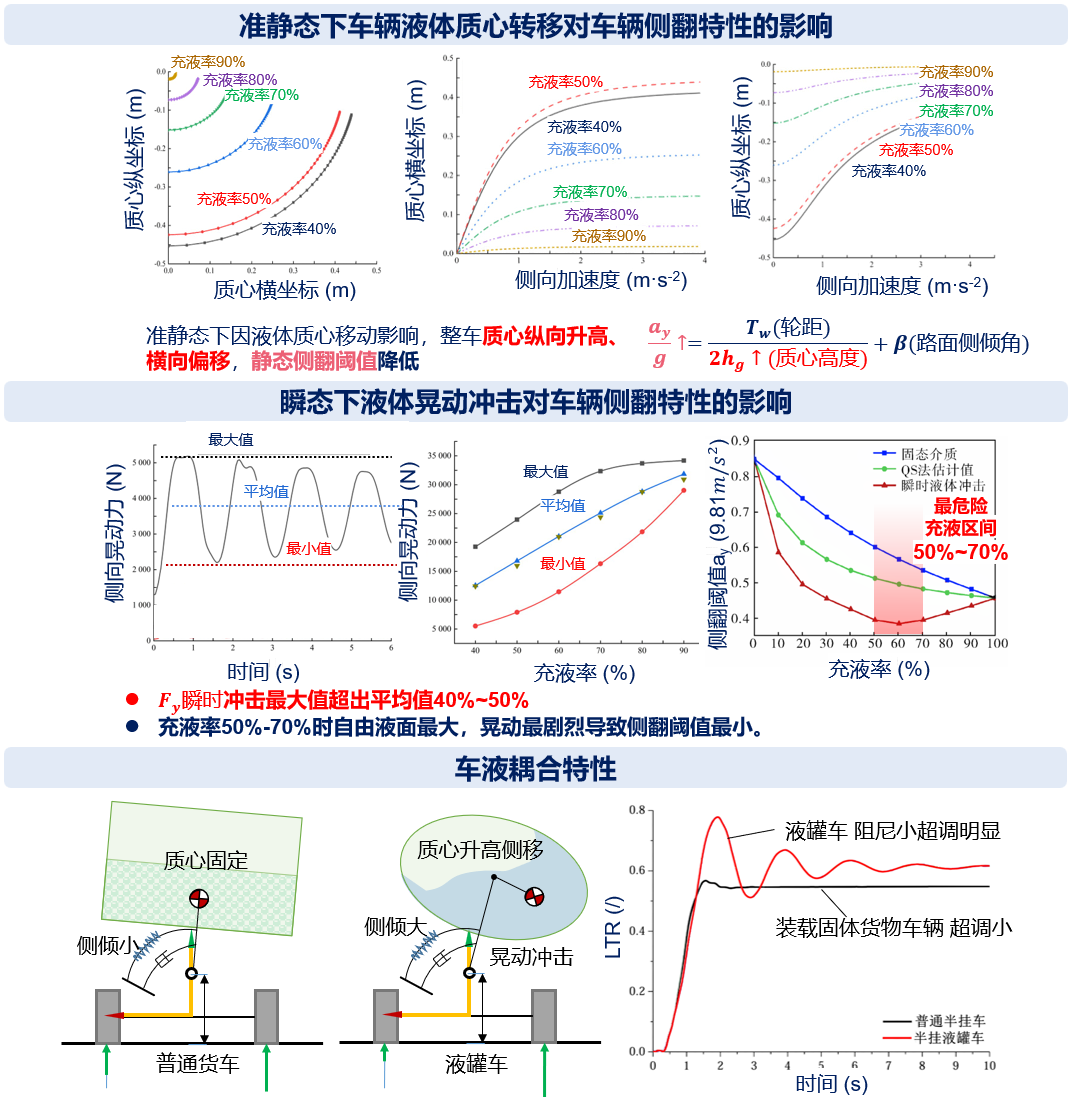
\includegraphics[width=1.0\linewidth]{fig/chap1/two_factors.png}
        \caption{车液耦合机理说明\cite{maohaijian2021fsi,huangyang2017impact,wangqiongyao2017sloshing,wanying2020antirolover}}
        \label{fig:vehicle_liquid_couple_mechanism}
      \end{figure}

      综合上述研究，车--液耦合对车辆侧向动力学的主要影响可概括为：\emph{(i) 响应幅值增大}（准静态质心迁移抬升等效侧倾力矩），\emph{(ii) 超调与峰值冲击显著}（瞬态晃动冲击引入额外侧向力/侧倾力矩），以及\emph{(iii) 阻尼偏小导致振荡持续}（流体等效阻尼有限且能量耗散慢）。这些特性共同解释了液罐车在中等充液率与强横向激励工况下更易出现侧倾失稳的现象。因此，后续建模方法的选择需在\emph{可解释的关键模态表达}与\emph{实时性}之间权衡。

    \subsubsection{液体晃动建模研究现状}
      \label{subsub:liquid_shaking_modeling}

      液体晃动建模最早主要服务于飞行器燃料箱（飞机油箱、火箭燃料箱等）、船舶配重水舱以及车辆油箱等场景，近年来逐步扩展至液罐车晃动与侧倾稳定性问题。针对晃动建模，学术界形成了多类方法体系。贾心红等\cite{jiaxinhong2022review}对相关方法进行了系统归纳，可概括为四类：\emph{准静态模型法}、\emph{机械等效力学模型法}、\emph{液体晃动动力学（流体）模型法}与\emph{实验研究法}（见图~\ref{fig:liquid_modeling_methods}）。

      \begin{figure}
        \centering
        \subcaptionbox{准静态模型法\cite{huangyang2017impact}\label{fig:liquid_model_qs}}
          {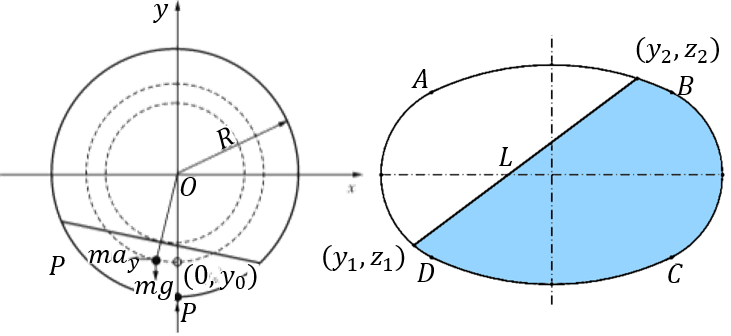
\includegraphics[width=0.48\linewidth]{fig/chap1/quasi_static.png}}
        \subcaptionbox{液体晃动动力学模型法\cite{maohaijian2021fsi,yuzhixin2018mpc}\label{fig:liquid_model_cfd}}
          {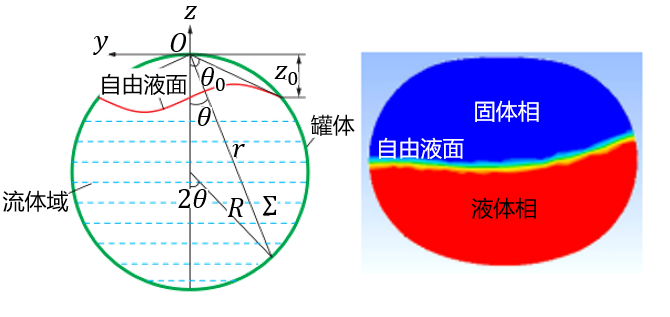
\includegraphics[width=0.48\linewidth]{fig/chap1/fluid_dynamic_model.png}}
        \subcaptionbox{实验研究法\cite{wangxiaorun2022lateralacc,wanying2020antirolover}\label{fig:liquid_model_experiment}}
          {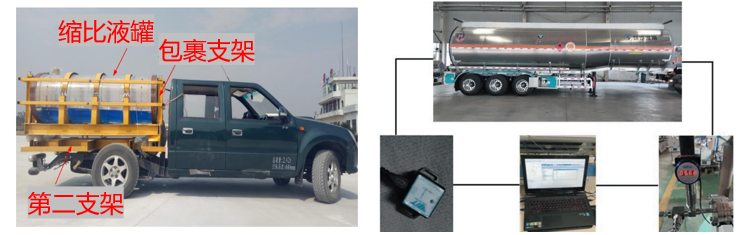
\includegraphics[width=0.48\linewidth]{fig/chap1/experiment_method.png}}
        \subcaptionbox{机械等效力学模型法\cite{yuzhixin2019optimalcontrol,zhaoweiqiang2018equivalent,zhaoweiqiang2019semitrailer}\label{fig:liquid_model_equivalent_model}}
          {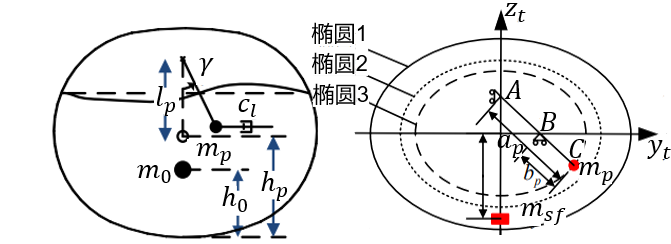
\includegraphics[width=0.48\linewidth]{fig/chap1/equivalent_model.png}}
        \caption{液体晃动建模方法}
        \label{fig:liquid_modeling_methods}
      \end{figure}

      \paragraph{(1) 准静态模型法（QS）}
      准静态模型（Quasi-Static Model, QS）主要描述稳态工况下自由液面与液体质心位置，忽略动态晃动过程，通常仅利用截面几何与静力平衡关系进行解析/半解析表达。该方法在稳态侧向加速度下对平均晃动力/侧倾力矩的估计具有一定有效性，但在变道、蛇形等瞬态工况下，由于晃动冲击与相位滞后显著，QS模型误差会明显增大。黄洋等\cite{huangyang2017impact}对比QS与CFD分析瞬态冲击，指出峰值冲击可显著高于平均值，并定义瞬时液体冲击影响因子以表征瞬态冲击导致侧翻阈值相对QS结果的折减；该因子在\SI{0}{\percent}与\SI{100}{\percent}充液率时为0，并在\SI{50}{\percent}附近达到最大（\SI{22.61}{\percent}）。何烈云等\cite{helieyun2020quasistatic}建立椭圆截面罐体的准静态等效模型，分析侧倾稳定性与截面形状、液体装载率等因素的关系，进一步说明QS方法在稳态设计与参数敏感性分析中的价值。

      \paragraph{(2) 机械等效力学模型法}
      机械等效模型以“输入输出等效”为原则，将液体系统视为黑箱，通过构造单摆、弹簧--质量--阻尼、多摆或椭圆规摆等机械系统来逼近液体晃动所产生的等效力/力矩。其优势在于\emph{计算实时性好、易于嵌入控制与规划}，并可在一定范围内准确描述一阶/低阶晃动；局限在于模型能表达的模态受结构形式限制，常难以覆盖水跃、飞溅等强非线性现象，且更高阶模态需要更复杂的等效结构。如图~\ref{fig:machenical}所示，Salem\cite{salem2000rollover}较早提出椭圆规摆（Trammel Pendulum, TP）用于液罐车液体建模，并指出其对椭圆罐体在较大侧向加速度范围内往往优于单摆模型。杨秀建等\cite{yangxiujian2018multimass}与吴相稷\cite{wuxiangji2018sloshingmodel}提出多质量椭圆规摆模型，并对比证明多质量结构可提升多工况下等效力拟合精度。戚笑景等\cite{Komasa2023observing}提出广义摆模型（Generalized Pendulum Model, GPM）概念，其中双质量椭圆规摆（DMTP）与组合双摆（TPSP）等可将二维晃动力特性的等效精度显著提升，并进一步提出为高精实时控制设计的包含侧向与侧倾双输入的单摆模型\cite{KomasaQi2025AntiRollover_TITS}。

      \begin{figure}
        \centering
        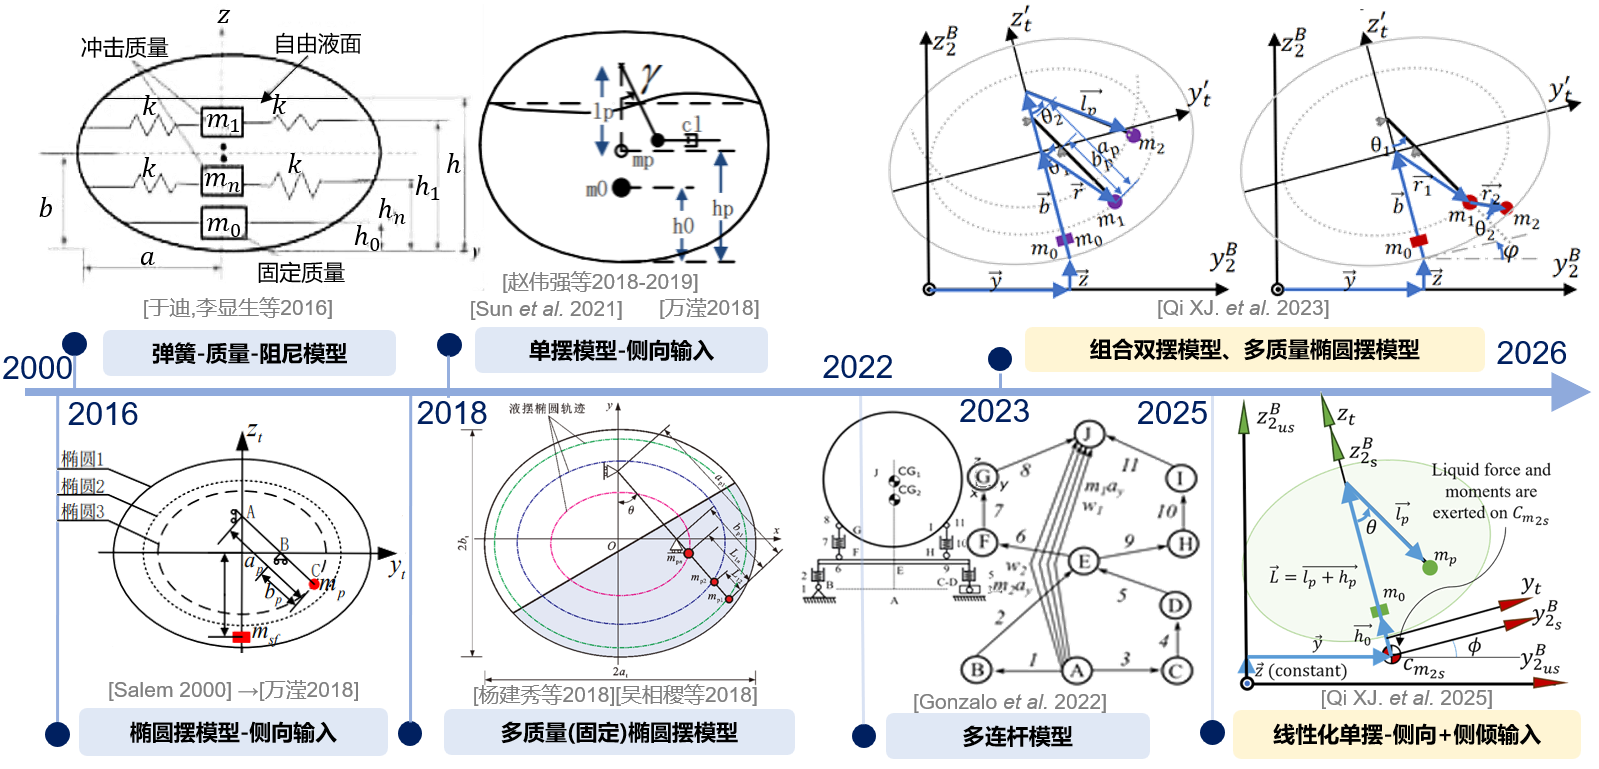
\includegraphics[width=1.0\linewidth]{fig/chap1/machenical.png}
        \caption{液体晃动机械等效模型发展}
        \label{fig:machenical}
      \end{figure}

      \paragraph{(3) 液体晃动动力学模型法}
      该类方法直接基于流体动力学微分方程描述液体流动，可在连续流体域或离散网格（有限体积/有限元等）内求解晃动响应，典型包括线性晃动理论与CFD数值方法。线性理论通常适用于简单几何与小幅晃动，推导复杂但有助于机理分析；CFD方法可捕捉强非线性、分离、飞溅等高阶现象，精度优势明显，且借助Fluent、StarCCM+等软件可较方便建模，但计算开销巨大，通常更适合作为高精度基准或离线标定工具，而不适用于实时控制系统的在线求解。

      \paragraph{(4) 实验研究法}
      实验研究可直观获取真实晃动行为与车辆响应，但受安全性与成本限制，涉及实车与真实危化品的高风险试验较少；多数工作基于相似性原理采用缩比液罐与台架/缩比实车平台验证模型与控制策略。王小润等\cite{wangxiaorun2022lateralacc}在室内场地借助台架辅助开展实车试验，并在约\SI{0.1}{g}侧向激励下与CFD结果对比验证线性晃动条件下CFD可靠性；万滢\cite{wanying2020antirolover}构建缩比液罐车模型并开展缩比实车实验，将测得的加速度作为CFD输入并与实验数据对比，验证联合仿真平台的一致性。

      综合比较四类方法：机械等效模型在能够表达低阶晃动的前提下具备较高实时性，因而更适用于车辆规划与控制；但其表达能力依赖等效结构设计，现有模型多聚焦于横向或纵向截面内的二维晃动，难以充分反映对车辆动力学同样重要的输出模态（例如横摆/俯仰方向的等效力矩），且往往忽略纵向加减速与横纵向流动耦合对横向晃动的影响，这为后续在复杂交通工况下的精确预测与鲁棒控制带来挑战。

    \subsubsection{液罐车动力学建模研究现状}
      \label{subsub:vehicle_dynamics}
      在规划与控制中引入液罐车动力学约束的前提是建立可用于计算的车--液耦合动力学模型。考虑工程应用的实时性需求，常见建模路线是以简化车辆横向/横摆模型为骨架，并与液体晃动模型（QS/等效力学/流体模型等）耦合形成低阶可计算模型。对整体式液罐车而言，车辆部分常采用自由度（Degree of Freedom, DOF）自行车模型或3DOF模型（纵向、侧向、横摆）与液体模型耦合；为刻画侧倾风险，也有研究引入包含侧倾自由度的4DOF模型，或以侧倾、横摆、侧向为核心的低阶模型与液体模型结合\cite{yudi2019rollstability}。任园园等\cite{renyuanyuan2020precisemodel}采用椭圆规摆近似液体并与3DOF车辆模型耦合，推导得到4DOF液罐车动力学模型，用于数值仿真分析液罐车相较固体载货车辆的运动学特性差异；Matthew等\cite{aquaro1999fem}基于有限元思想离散罐体质量，使用梁单元与单摆分别描述车体与液体；万滢\cite{wanying2020antirolover}采用椭圆规摆进行液体建模，并进一步用等效单摆分别与3DOF与4DOF车辆模型耦合，为LQR抑晃与防侧翻控制提供模型依据。

      对于半挂液罐车，由于牵引车与挂车通过铰接耦合，完整动力学模型可包含牵引车与挂车的平面运动（纵向、侧向、横摆）以及侧倾、俯仰等多自由度，维数较高；在现有研究中通常按研究目标进行简化。常见的车辆简化模型包括：牵引车纵向、侧向、横摆加挂车横摆的4DOF模型（如制动工况分析\cite{heren2016braking}），以及牵引车侧向、横摆、侧倾加挂车横摆、侧倾的5DOF模型\cite{zongchangfu2014identification,niezhigen2015heavyduty}等。于志新等\cite{yuzhixin2018mpc,yuzhixin2019optimalcontrol}基于势流理论建立液体晃动方程，并与5DOF半挂车动力学模型耦合，构建了6DOF半挂液罐车模型，体现了“车辆简化模型 + 可计算液体模型”的主流路线。

      获得模型结构后，\emph{参数辨识}是决定模型可用性的关键环节。常用做法是基于最优化搜索（遗传算法、粒子群等）最小化模型输出与高精度仿真/实验输出之间的误差以估计参数。万滢\cite{wanying2020antirolover}利用遗传算法对等效单摆与椭圆规摆模型进行参数拟合，使其匹配\SI{1}{m/s^2}侧向激励下CFD的侧向力输出；Yu等\cite{yudi2016nonfull}对比不同突变率与种群规模配置下遗传算法的辨识性能，指出当种群规模较小（如小于80）时突变率过大或过小均可能导致最优性下降。对于车辆部分参数，宗长富\cite{zongchangfu2014identification}与聂枝根等\cite{niezhigen2015heavyduty}采用“双模型 + 遗传算法”的方式进行多工况辨识，并建立参数插值表以适配运行时工况变化。

      总体而言，半挂液罐车的工程化建模常以5DOF左右的半挂车动力学简化模型为基础，叠加可实时计算的液体晃动模型（其中线性化单摆/椭圆规摆等机械等效模型最常见），在精度与实时性之间取得折中；但现有模型多仍存在横纵向耦合不足、输出模态受限以及在复杂交通工况下泛化能力有限等问题，为后续面向预测性规划与鲁棒控制的模型升级提供了明确方向。

  \subsection{液罐车防侧翻主被动安全措施研究现状}
    通过液罐车自身的改进解决其侧倾稳定性差问题的思路有两大类，一类是以改进车辆自身性能的被动措施；另一类是从控制入手的主动安全措施，下面对两种思路分别介绍。
    \subsubsection{液罐车防侧翻的被动安全措施研究现状}
    \label{subsub:passive_safty}

      被动防侧翻措施主要从\emph{车辆结构与罐体内部构型}入手，通过改变液体晃动模式、降低液体质心迁移幅度、改善罐体受力路径等方式提升侧倾稳定性。现有研究与工程实践中，典型被动措施如图~\ref{fig:passive_methods}所示，包括：\emph{罐体形状（尤其截面形状）优化}、\emph{防浪板/防波板设计}以及\emph{固定自由液面或抑制晃动的装置（如弹性气袋）}等。

      罐体截面形状直接影响液体质心位置及其在横向激励下的迁移规律，从而影响侧倾稳定性。陈益苞等\cite{chenyibao2016crosssection}建立了相同面积的圆形截面、两种改进椭圆形截面以及三种锥形截面的QS模型，对比了不同充液比下多种侧倾稳定性指标，验证其提出的部分锥形截面在提升侧倾稳定性方面具有优势。瞿绘军等\cite{quhuijun2017calculation}依据GB28373-2012《N类和O类罐式车辆侧倾稳定性》\cite{gb28373_2012}的计算方法，并以GB7258-2017《机动车运行安全技术要求》\cite{gb7258_2017}的稳定性判定条件为依据，对某型号液罐车进行理论计算，指出变截面罐体相较非变截面罐体可降低质心高度，且在设计许可范围内变截面高度越大整车重心越低。于迪等\cite{yudi2016nonfull}建立$n$阶弹簧--质量等效模型描述罐体线性横向振动模态，研究不同椭圆率罐体后指出椭圆率$a_{t}/b_{t}=1.5$时侧向冲击力与侧倾力矩较小。进一步地，Di Yu等\cite{yudi2019rollstability}利用遗传算法优化椭圆规摆等效模型参数以最小化侧倾力矩，发现当$a_{t}=\SIrange{1.6}{1.7}{m}$、$b_{t}=\SIrange{1.15}{1.25}{m}$（即$a_{t}/b_{t}=\SIrange{1.28}{1.478}{}$）时稳定性较优；李显生\cite{lixiansheng2015ga}亦采用遗传算法优化椭圆率并以液体质心高度与侧倾力矩为目标，得到最优椭圆率约为1.367。

      通过设置防浪板抑制液体横向流动是工程上常见且有效的被动手段。Guillermo等\cite{moreno2022davies}采用质点簇--杆件等效模型研究液体质心迁移与车辆侧倾稳定性之间的关系，提出新的稳定性指标，并给出“抑制液体侧向流动的装置可提升侧倾稳定性”的结论。刘奎等\cite{liukui2009braking,liukui2009steering}通过CFD仿真分析制动与转向工况，指出纵向防波板有效面积大于横截面\SI{40}{\percent}时可有效改善受力，并给出按容积间隔布置纵向防波板的工程建议；同时，纵向防波板的设置也与现行安全规程的设计要求相一致。相比之下，横向防波板由于缺乏统一规定且制造成本较高，工程应用中较少采用。

      除上述两类主流方向外，研究还探索了通过弹性气袋等装置固定自由液面以抑制晃动\cite{wangqiongyao2017sloshing}、通过罐体结构改进优化受力\cite{fangliang2022fe}、以及利用地理信息系统提供道路结构预警信息\cite{zhangweihua2019gist}等思路，以从液体晃动、结构强度或驾驶辅助层面降低翻车风险。

      \begin{figure}
        \centering
        \subcaptionbox{改进液罐截面\cite{chenyibao2016crosssection}\label{fig:cross_sec_improve}}
          {
\includegraphics[width=0.31\linewidth]{fig/chap1/tank_shape.png}}
        \subcaptionbox{改进防浪板形状\cite{hanyoubin2019vof}\label{fig:wave_board_improve}}
          {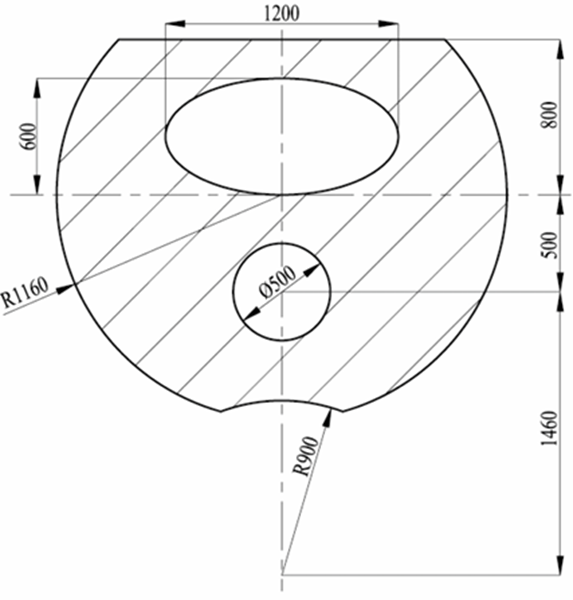
\includegraphics[width=0.31\linewidth]{fig/chap1/wave_proof.png}}
        \subcaptionbox{增加弹性气袋\cite{wangqiongyao2017sloshing}\label{fig:elastic_bag}}
          {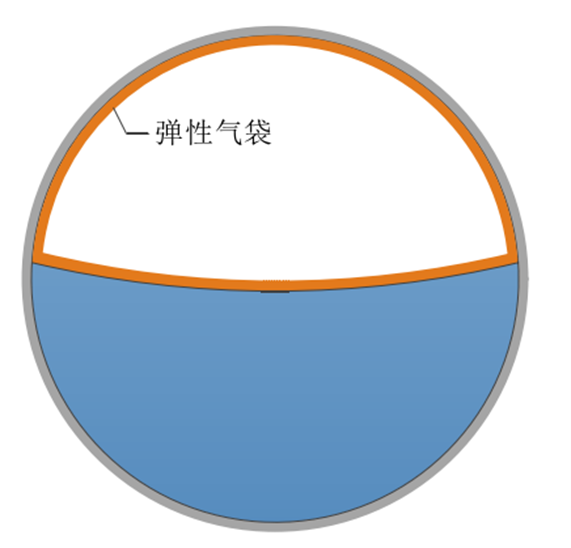
\includegraphics[width=0.31\linewidth]{fig/chap1/elastic_bag.png}}
        \caption{液罐车防侧翻被动安全措施}
        \label{fig:passive_methods}
      \end{figure}

      综上，被动安全措施围绕罐体形状、防浪结构与自由液面抑制等方面已形成较为系统的研究与工程应用。受限于整车成本、轻量化、检修/清洗便利性等约束，罐体内部难以引入过于复杂或维护成本高的构件，使得多数“可产业化”的方案在边界工况下仍存在剩余风险。现实事故中，液罐车侧翻往往还与道路几何突变（如小半径弯道、纵坡叠加）、驾驶员对风险感知滞后、对周车动态预测不足或违规操作等外部因素耦合有关。因而，在车路云一体化推进的大背景下，若能在车云协同架构下将主动风险预测、预防性轨迹规划与控制干预结合，有望在进入危险状态之前降低侧翻风险，并与被动措施形成互补的分层安全体系。
   
            
    \subsubsection{液罐车防侧翻主动安全措施研究现状}
    \label{subsub:active_safty}

      面向液罐车的主动防侧翻方法总体可归纳为两条互补路径：\emph{防侧翻运动规划}与\emph{防侧翻控制}。前者通过在决策与轨迹层提前约束侧向激励、侧倾响应及其演化过程，从源头降低车辆进入危险状态的概率，更偏向“预防”；后者则在车辆已处于高侧翻风险状态时，通过执行器施加控制作用抑制侧倾失稳，更偏向“救车”。考虑本文对象为半挂式液罐车，其防侧翻问题同时受到半挂结构、液体晃动耦合及自动驾驶执行条件的共同影响，因而有必要分别从防侧翻运动规划与防侧翻控制两方面进行综述。

      \subsubsection*{(1) 防侧翻运动规划研究现状}

      防侧翻运动规划的核心在于：在轨迹生成阶段显式限制可能诱发侧翻的横向激励与姿态响应。因此，无论采用何种规划方法，首先都需要回答“如何衡量侧翻风险”这一基础问题。现有研究中常用的侧翻风险指标包括：基于质心高度与轮距的静态稳定因数（Static Stability Factor, SSF）\cite{huston2014ssf}、动态稳定因数（Dynamic Stability Factor, DSF）\cite{jin2007critical,heyuancha0_2010factor}、侧向载荷转移率（Lateral-load Transfer Ratio, LTR）\cite{zhang2016pulsed,zhao2019hinfty}及其变体\cite{jin2021heavytruck}、多参数联合指标\cite{jin2016tripped,jin2019triaxle,imine2015switched}、侧翻时间（Time to Rollover, TTR）\cite{wanying2020antirolover,zeng2017bpnn}以及零力矩点（Zero Moment Point, ZMP）\cite{jinliqiang2017yujing}等。SSF物理意义清晰但难以反映动态侧翻过程；DSF涉及参数较多且对工况敏感；LTR物理意义直观、与轮胎接地载荷关联紧密，是目前较常用的动态防侧翻指标，但往往需借助悬架力等量进行等效估计；TTR更适用于风险预警与触发逻辑设计；ZMP在车辆侧翻研究中的应用相对较少。上述指标不仅决定了规划器如何定义“危险”，也直接影响其约束构造方式与代价函数形式。

      在此基础上，现有防侧翻运动规划通常是在通用轨迹规划框架中进一步引入车辆侧倾动力学约束或风险代价，以限制侧向加速度、横摆响应及载荷转移峰值。现有通用轨迹规划方法大体可概括为五类：基于搜索、基于采样、基于几何参数化、基于优化以及基于学习的方法。

      基于搜索的方法常见有Dijkstra\cite{bacha2008odin}、A*\cite{likhachev2009planning}、Hybrid A*\cite{kurzer2016hybrida}、D*\cite{stentz1994efficient}、分阶段动态规划（Dynamic Programming, DP）\cite{dong2023ecocruising}以及结构化道路离散搜索的Lattice Planner\cite{werling2010frenet}等。该类方法通常具有较好的完备性，但由于依赖状态空间离散化，往往难以充分刻画车辆连续动力学、执行器约束及侧翻风险连续演化过程。

      基于采样的方法如PRM\cite{kuwata2009realtime}、RRT\cite{karaman2011sampling}、RRT*\cite{klemm2015rrtconnect}、双向RRT*\cite{fan2024birrt}等，在复杂环境中具有较强的可行域搜索能力，适用于障碍物分布复杂或非结构化场景；但其生成结果受随机性影响较大，一致性与可重复性相对较弱，若进一步叠加侧翻约束，则常面临实时性与稳定性之间的折中。

      基于几何参数化的方法通过预设曲线形式直接生成满足连续性要求的候选轨迹。低速场景中常用Dubins曲线\cite{siedentop2015dubins}、Sine曲线\cite{huang2022sineresistance}等；高速场景中则常用回旋曲线/欧拉螺线\cite{brezak2014clothoids}、空间坐标多项式\cite{petrov2014overtaking}、贝塞尔曲线\cite{rastelli2014continuouscurvature}、非均匀B样条\cite{phanhuu2021bsplines}、样条曲线\cite{gotte2018splinebased}及PCHIP三阶插值\cite{hegedus2020realtime}等。这类方法计算代价较低，易于保证曲率连续，适合作为防侧翻轨迹形状约束的基础，但对复杂约束和多目标权衡表达能力有限。

      基于优化的方法通过显式优化控制输入或轨迹参数生成光滑轨迹，并将碰撞约束\cite{dong2023ecocruising}、人工势场\cite{liuzhiqiang2017shichang}以及LTR/TTR等风险指标纳入目标函数或约束条件。例如，Rasekhipour等\cite{rasekhipour2017pfmpc}构建三维虚拟势场并采用多约束MPC跟踪；Jin等\cite{jin2021heavytruck}利用悬架力等效的LTR防侧翻代价构建NMPC控制器并结合人工势场避障；Cheng等\cite{cheng2019longitudinal}对采样轨迹按LTR侧翻代价进行筛选，并采用五次多项式平滑后执行；Li等\cite{li2019rollover}在时空占用网格上搜索LTR侧翻代价最小的轨迹。相较于前述方法，优化方法更易将防侧翻约束、避障约束与舒适性、可执行性等目标统一到同一框架之中，因此是当前防侧翻规划研究的重要方向。

      基于学习的方法通常采用强化学习（Reinforcement Learning, RL）\cite{wu2024rlsurvey,zhang2023intersectionrl,irshayyid2024highwayrl}，并与Safe RL理论\cite{zhang2024saferl_tits,gu2024saferl_tpami,garcia2015saferl}结合，以期在复杂交互环境中自动学习兼顾安全与效率的行为策略。此类方法理论上具备较高上限与较强场景适应性，但训练高度依赖数据质量、场景覆盖和奖励设计，且在实际驾驶任务中仍可能表现出过度保守或安全性不足的两端化问题，目前仍处于快速发展阶段。

      对于半挂式液罐车而言，防侧翻规划问题还具有区别于普通单体车辆的额外复杂性。首先，半挂结构导致牵引车与挂车存在“不同轨”现象，规划时不仅要考虑牵引车本体避障，还必须同时满足挂车对静态与动态障碍物的避障要求；其次，除普通车辆常见的曲率、横向加速度与轮胎附着约束外，半挂车还需额外考虑防折叠、铰接角稳定性以及牵挂协同跟踪等约束；进一步地，对于液罐车，液体晃动会与车辆横摆、侧倾和路径变化相互耦合，使得轨迹规划不再只是几何可行或动力学可行问题，而是同时受到液体动力学影响的强安全约束规划问题。

      现有半挂车规划与跟踪研究可为该问题提供一定基础。低速工况主要对应自动泊车，规划层通常基于半挂车运动学模型，同时考虑牵引车与挂车避障，采用搜索、采样、优化或强化学习等方法规划牵引车轨迹，控制层则通过牵引车或挂车一侧的跟踪实现整体约束满足。例如，王元民等\cite{wangyuanmin2024}将二次规划（Quadratic Programming, QP）与双向拓展快速随机树（Bi-RRT）结合求解初始解，并通过偏向性采样平滑实现半挂车避障倒车；陈朝\cite{chenchao2023}结合铰接角与碰撞约束进行B样条优化实现垂直泊入；贾生超\cite{jiasenchao2023}推导前向/后向铰接角稳定条件并与混合$A^\ast$结合实现自动泊车。高速工况下，半挂车轨迹规划往往弱化低速场景下突出的内轮差问题，更强调在满足高速稳定性要求的前提下进行轨迹生成与协同跟踪。例如，李斯旭等\cite{lisixu2021}结合多点预瞄与状态轨迹线性化加权牵引车与挂车侧向跟踪误差；曹莉凌等\cite{caoliling2024}利用LQR调节铰接角误差并以PID进一步补偿；张发旺等\cite{zhangfawang2025}提出双策略跟踪框架，上层用近似动态规划（Approximated Dynamic Programming, ADP）控制牵引车跟踪，下层用IPOPT优化权重以降低挂车跟踪误差；宋广昊\cite{songguanghao2023}提出羊角螺线接贝塞尔曲线的两段式换道轨迹以降低峰值LTR，并结合挂车轴转向实现挂车轨迹跟踪；王洪昌\cite{wanghongchang2023}提出基于同伦流形的混合A*/DP规划方法，实现路口离散化后的快速半挂车避障规划。

      总体来看，现有研究一方面已形成较丰富的通用防侧翻规划方法及风险指标体系，另一方面也积累了半挂车规划与跟踪的相关研究基础；但公开文献中仍缺少真正面向\emph{半挂式液罐车}特性的防侧翻运动规划方法。具体而言，现有普通车辆防侧翻规划多未考虑牵挂结构与液体晃动耦合，而现有半挂车规划研究又多聚焦避障、泊车或一般高速跟踪，缺少将液体晃动、半挂结构特性与强侧翻约束统一纳入规划器的研究。因此，针对半挂式液罐车构建面向自动驾驶场景的防侧翻运动规划方法，仍存在明显研究空白。

      \subsubsection*{(2) 防侧翻控制研究现状}

      与防侧翻运动规划从源头降低风险不同，防侧翻控制更强调在车辆已进入危险状态或接近危险边界时，利用执行器快速干预侧倾动态。现有车辆防侧翻控制方法总体上可归纳为四条主要技术路线：主动悬架、差动制动、分布式驱动和转向控制，以及它们的组合形式\cite{xu2011rollover,liang2022multiagent}。

      主动悬架通过调节左右悬架支撑力直接抑制车身侧倾，是对侧翻状态作用最直接的一类手段\cite{xiao2020rollsuspension}。其优势在于能够直接作用于侧倾自由度，但局限在于硬件与能耗成本较高，且在极端工况下抑制能力仍受限，商用车规模化部署难度较大。差动制动通过左右轮制动力不均产生附加横摆力矩，进而间接影响侧倾动力学\cite{carlson1981two}。该方法可基于现有ESP等硬件体系较低成本实现，工程可落地性较好，但由于其通过“横摆力矩$\rightarrow$横向运动$\rightarrow$侧倾响应”的间接路径发挥作用，对侧倾状态的控制能力存在先天上限。分布式驱动可视为差动制动的扩展，通过多个车轮独立施加驱动/制动力增强可用横摆力矩\cite{zilin2023integrated}，但通常依赖轮毂电机或带动力挂车等特殊结构，实际应用范围较窄。转向控制则通过调节前轮和/或后轮转角改变车辆路径和横向激励，其本质上可视为在控制层实施的路径再规划\cite{shao2023vhrobustmpc}。与差动制动相比，转向控制对侧翻风险的抑制更为主动，在极限工况下通常具有更强的翻车避免潜力，但对转向执行器能力、路径可行空间及控制设计均提出更高要求。

      \begin{figure}
        \centering
        \subcaptionbox{主动悬架\label{fig:active_suspension}}
          {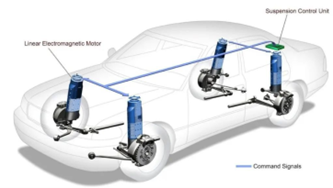
\includegraphics[width=0.40\linewidth]{fig/chap1/active_suspension.png}}
        \subcaptionbox{转向控制(前轮和/或后轮)\label{fig:active_steering}}
          {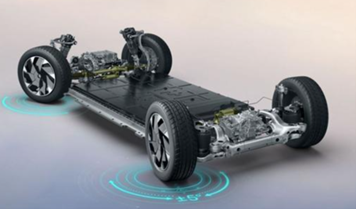
\includegraphics[width=0.40\linewidth]{fig/chap1/active_steering.png}}
        \vspace{0.2cm}
        \subcaptionbox{差动制动\label{fig:diff_braking}}
          {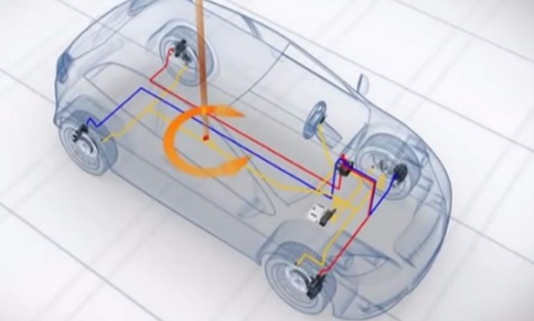
\includegraphics[width=0.40\linewidth]{fig/chap1/diff_braking.png}}
        \subcaptionbox{分布式驱动\label{fig:distributed_driving}}
          {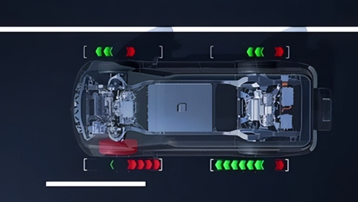
\includegraphics[width=0.40\linewidth]{fig/chap1/dist_driving.png}}
        \caption{现有车辆防侧翻控制方法}
        \label{fig:anti_rollover_methods}
      \end{figure}

      对于液罐车而言，防侧翻控制研究总体上仍是一个相对小众的方向。2018年以来，国内外公开文献中相关工作数量虽有所增加，但总体规模仍较小，且大多面向人工驾驶条件下的主动安全辅助驾驶。受限于车载硬件条件与工程可实施性，现有液罐车防侧翻控制研究主要集中于差动制动、转向控制及两者组合，主动悬架与分布式驱动在该领域中的研究和应用相对较少。

      在建模层面，现有研究通常采用等效摆模型或势流模型描述液体晃动，并与车辆横向动力学模型耦合；在控制方法层面，则多采用比例积分微分控制（Proportional--Integral--Derivative, PID）及模糊PID、线性二次型调节器（Linear Quadratic Regulator, LQR）、模型预测控制（Model Predictive Control, MPC）、无模型自适应控制（Model-free Adaptive Control, MFAC）\cite{huyun2019mfac,luoyugong2019sbw,tangzeyue2023mpcmfac,fengzengxi2021mfacpso}、$H_\infty$控制\cite{zhao2019hinfty}等。

      从研究演进看，赵伟强、封冉等\cite{zhaoweiqiang2018equivalent}较早建立等效单摆与3DOF液罐车辆耦合模型，并采用PID控制差动制动实现防侧翻，形成了“液体摆模型 + 差动制动救车”的早期研究范式。于志新、程新新等\cite{yuzhixin2018mpc}进一步基于势流理论建立液体晃动模型，并与半挂液罐车模型耦合，采用MPC同时协调差动制动与转向控制，体现了由单一执行器向多执行器协同发展的趋势。随后若干研究沿这一框架展开拓展，例如赵伟强、凌锦鹏等\cite{zhaoweiqiang2019semitrailer}将等效单摆与6DOF半挂液罐车模型耦合并采用LQR进行差动制动控制；于志新等\cite{yuzhixin2019optimalcontrol}同样将势流液体模型与6DOF半挂车结合并采用LQR控制；Sun等\cite{Reviewer2_SunWencai2022}将单摆与3DOF车辆结合并基于LQR误差模型实现侧倾稳定性控制；万滢\cite{wanying2020antirolover}以TTR为指标，基于等效单摆与3DOF车辆模型构建横摆--抑晃--防侧翻最优控制系统。与早期研究普遍采用机械等效模型进行算法验证不同，李杰等\cite{lijie2020carliquid}通过在Fluent中加入自定义动量源项实现车--液耦合仿真，万滢\cite{wanying2020antirolover}则进一步将CFD仿真用于平台及方法验证，提高了液体动力学验证精度。

      在控制手段比较方面，Li等\cite{MFAC_LiXiansheng2021}分别为差动制动与转向控制设计MFAC，并指出转向控制在稳定时间与超调方面均优于差动制动，在多种工况下峰值LTR降低更为显著；郑雪莲等\cite{zhengxuelian2019mfacpatent}提出基于FFDL-MFAC的侧翻稳定性控制方法，无需精确动力学模型即可通过附加差动制动控制横摆角速度，具有一定模型鲁棒性。这与已有研究认识一致：横摆力矩对侧倾动力学的影响通常是间接且受限的\cite{liutianfeng2024heterogeneous}，而转向控制通过直接改变车辆路径和横向激励，在极限工况下往往具有更强的翻车避免能力。

      近年来，随着自动驾驶液罐车研究的推进，部分工作开始将防侧翻控制从传统辅助驾驶场景扩展到无人驾驶场景。魏星\cite{weixing2023_antirollover}提出面向半挂式液罐车的防侧翻与路径跟踪协调控制方法，将主动防倾杆、差动制动与轨迹跟踪控制通过状态机切换实现多模态控制，体现了由单一“救车控制”向“常态运行 + 临险干预”结合的思路演进。然而总体来看，现有方案仍大多建立在横纵向解耦、液体模型简化及局部控制层补偿的基础上，较少从自动驾驶任务出发系统处理液体横纵向耦合流动、轨迹规划与执行协同以及复杂验证闭环等问题。

      综上分析，现有液罐车防侧翻控制研究已在执行器选择、液体建模、控制方法及验证手段等方面取得一定进展，但总体上仍以\emph{紧急救车}和\emph{事后抑制}为主，更多关注车辆已经进入高风险状态后的快速纠偏，而对自动驾驶条件下更为重要的\emph{预防性安全保障}关注不足。悬架力控制作用最直接但成本高，差动制动工程可实施性好但对侧倾的作用间接且上限有限，转向控制则在极限工况下展现出更强潜力。因而，若能将转向控制、差动制动等执行手段与防侧翻运动规划进一步协同设计，在进入危险区域之前就主动降低侧翻风险，并在临险时快速补充控制，有望显著提升半挂式液罐车主动安全系统的整体有效性。




  \subsection{车云协同预测性决策与规划研究现状}

    云端预测性行为决策与运动规划是在单车自动驾驶决策与规划的基础上发展而来的，相对于单车方案，云端预测性的决策和规划更加考虑了云端的全局感知、并行算力与协同优化优势，对单车所触及不到的长时域规律进行解析，并给出更具指导性的建议。

    \subsubsection{单车智能行为决策及其向云端的拓展}
      \label{subsub:autonomous_decision}

      尽管云端与车端在可用信息量、更新频率与规划颗粒度上存在差异，其决策与规划的基本范式是相通的：在不确定、多主体交互的交通环境中，生成既安全又高效且可执行的行为与轨迹。因此，较为成熟的单车智能行为决策为云端预测性决策提供了重要参考。行为决策自始至终试图解决的核心问题只有一个：\emph{如何处理自车与周围交通参与者之间的交互}，如图~\ref{fig:pred_dec_int}所示。

      自DARPA自动驾驶挑战赛以来，感知--预测--决策--规划--控制的模块化流程被沿用多年\cite{ferguson2008urban,urmson2008boss,leonard2008perception,kammel2008annieway,vonhundelshausen2008tentacles,montemerlo2008junior,thrun2006stanley}，但该流程隐藏了一个关键逻辑矛盾：若先对周车进行预测再据此决策，则预测结果默认与自车决策无关；而实际交通中周车行为往往会对自车动作产生反应，预测应当随自车候选决策而变化。由此，传统“先预测后决策”的串行结构在多车交互场景下容易出现保守、迟滞或不稳定等问题。为修正上述矛盾，近年来模块化路线的一个共同趋势是\emph{预测--决策一体化}。
      
      现有模块化方法大体可按交互处理方式划分为显式交互、隐式交互及综合式交互三类。\emph{显式交互}以自车候选策略/意图划分场景，在每个候选行为下预测周车反应，并对不同候选行为的长期收益与风险进行比较，典型代表为多策略决策方法（Multi-Policy Decision Method, MPDM）；\emph{隐式交互}侧重对周车意图/不确定性构造多个可能情景，并在情景集合上评估自车应对策略，典型代表包括防御性规划（Contingency Planning）\cite{salvado2016contingency}与博弈论方法；\emph{综合式交互}将显式交互与隐式交互思想融合，并常与风险度量、礼貌性或协同性等机制结合。本文在附录\ref{sub:pipeline}中对模块化路线作进一步综述。
  
      端到端方案则进一步通过通过学习从环境表征到行为/轨迹的可微分联合映射，在训练阶段将预测、决策与规划的耦合显式纳入优化目标，从而缓解传统“先预测后决策”带来的交互一致性问题。常见实现包括基于模仿学习的端到端轨迹生成、基于强化学习的交互策略学习，以及以扩散/生成模型为代表的多模态规划生成等。端到端方法中最早发展起来的两端式端到端融合预测--决策--规划三者，近年来涌现的一段式端到端则将感知--规划的闭环打通，其中VLA方案则将感知--控制全链路打通。本文在附录\ref{sub:end2end}中对端到端路线作进一步综述。

      \begin{figure}
        \centering
        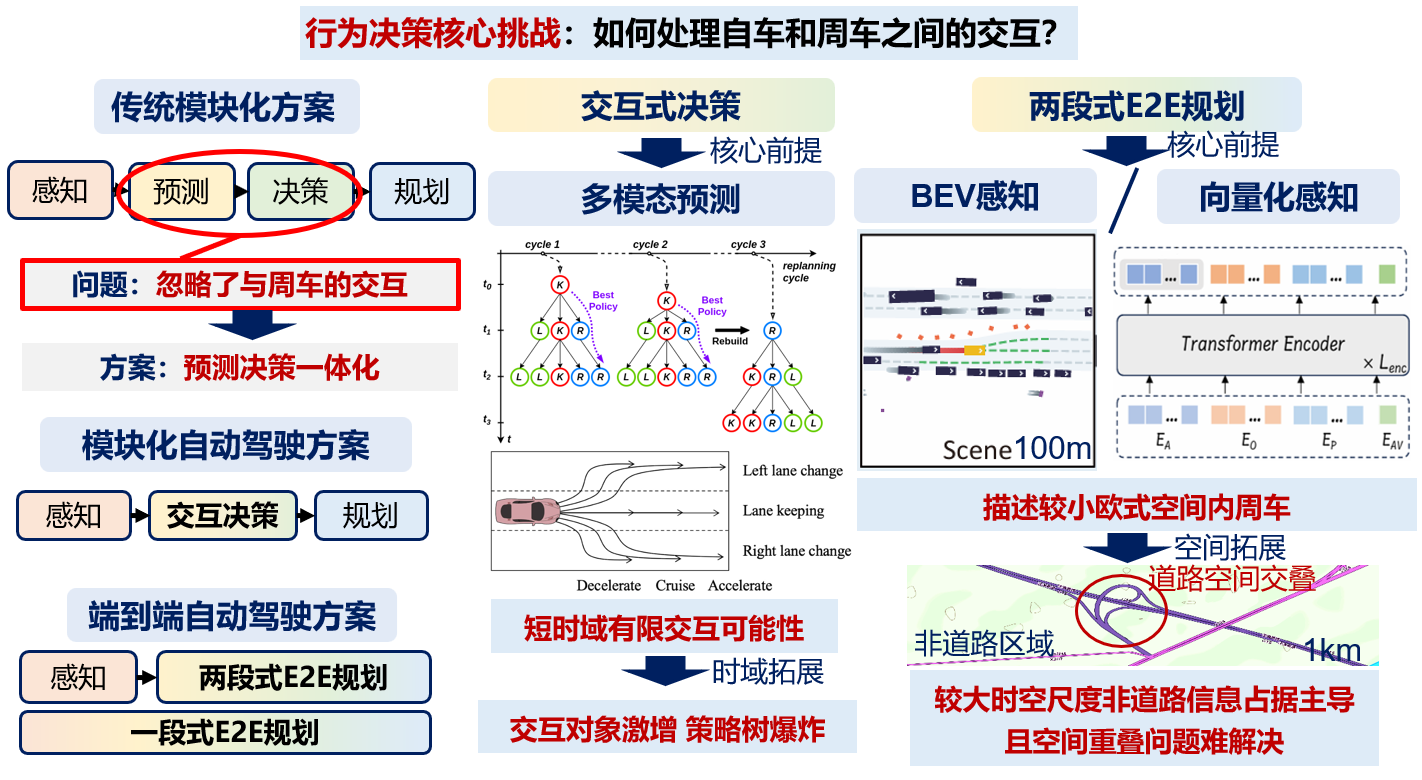
\includegraphics[width=1.0\linewidth]{fig/chap1/pred_dec_int.png}
        \caption{预测决策一体化思想及其向云端的拓展}
        \label{fig:pred_dec_int}
      \end{figure}
  
      对云端预测性行为决策而言，预测决策一体化的核心思想同样适用，但现有单车方案向云端长时域大空间尺度的拓展存在挑战。模块化方案的交互式决策需具备多模态周车预测能力从而据其构建自车行为树，但随云端时域与空间尺度的增加，周车行为树的规模将呈指数级增长，导致计算复杂度过高，且预测结果无法穷尽所有可能，即每次交互将忽略大量小概率时间，而这在长时域多次交互后将导致不确定性传播的严重失真；由于车云通信时延，端到端方案在云端通常采用两段式，其依赖的BEV感知特征或向量化感知适合描述小欧式空间内周车，在面对大时空尺度拓展时则包含大量无用非道路语义向量子空间，导致表征与计算效率低下。

      % 在得到行为/意图层决策后，运动规划模块需生成一条可跟踪的三维时空轨迹或二维平面路径。对于高速运动、安全敏感且多主体实时交互的结构化道路任务，通常需要对轨迹进行规划与跟踪。对非学习类方法而言，轨迹规划的差别主要体现在求解维度与约束处理方式：自动驾驶一般考虑车辆在平面内二维运动，故轨迹规划涉及三维时空求解。针对三维时空轨迹规划，现有研究可分为时空解耦规划与时空联合规划两类路线。

      % 时空解耦思路将三维规划拆解为两个二维规划问题。代表性案例如百度Apollo的EM-Planner\cite{fan2018apollo}采用横纵向解耦：先规划路径，再在ST图中进行碰撞检测，利用动态规划（Dynamic Programming, DP）求解离散空间中的速度曲线，并通过二次规划（Quadratic Planning, QP）进行平滑。该类方法计算效率高，但由于忽略横纵向耦合可能损失最优性。时空联合规划在计算上更昂贵，但不人为限制解空间，尤其对体积较大、可行解更少的商用车，往往能获得更优解。现有工作通过在策略参数空间优化\cite{tusimple2023aiday}、在不同自车--周车意图组合情景下联合优化\cite{li2023marc}、或引入同伦轨迹构型\cite{degroot2024topology}等方式开展时空联合规划。

      综上，单车自动驾驶的行为决策普遍通过预测--决策耦合的方式高效建模自车与周车的短期交互以规避先预测后决策的逻辑谬误，云端预测决策一体化势在必行。然而，现有适用于单车的交互建模方式难以拓展到需要考虑较大时空尺度的云端，亟需适用于云端的反映交互不确定性在长时域扩散的交互建模方法。

    \subsubsection{云控预测性决策与规划研究现状}
      \label{subsub:cloud_control}

      上一小节指出，单车自动驾驶决策与规划虽然能够较好处理短时局部交互，但仍受限于\emph{局部可观测、短时域预测与车端算力约束}，难以充分利用更大空间范围的信息开展长时域风险预判与协同行为组织。为此，车路云一体化系统在车端实时闭环之外，引入基于路侧、边缘侧或云端的并行决策与规划闭环：车辆继续负责本地高频感知、规划与控制，基础设施侧则利用更广域感知与更强计算资源，提供预测性决策建议、约束或目标，从而在\emph{不替代车端安全闭环}的前提下提升系统安全性、通行效率与能耗表现。

      从体系结构看，现有云控预测性决策与规划研究大体可归纳为三类：\emph{车端决策辅助}、\emph{车云分层控制}和\emph{云端全局/集中控制}\cite{Huang2025V2X}。三类架构在功能分配、协同深度、通信依赖与工程适用性方面存在明显差异。

      车端决策辅助以\emph{“车端为主、协同信息增益”}为基本思路，即利用V2X提供的他车、路侧或基础设施感知信息增强车端环境理解、行为预测与规划求解，但最终决策与执行仍由车辆本地完成。该类方法通常不改变单车自动驾驶原有闭环结构，而是在感知、预测或语义理解等环节引入外部信息以提升车端决策质量。代表性研究包括：UniV2X\cite{UniV2X2024}以车端规划为核心，将路端感知信息作为增量观测融入车端规划流程；UniMM-V2X\cite{UniMM_V2X2025}进一步在感知与预测环节解耦并行建模，在决策阶段融合车路两端预测结果以增强复杂交互理解；V2X-VLM\cite{V2X_VLM2025}引入大模型语义理解能力，使协同信息进一步服务于意图推断、交互解释与可执行规划生成。除单车规划增强外，车路信息也被用于局部多车协同决策与规划控制一体化设计，例如以路侧单元为中心的匝道汇入多智能体强化学习决策\cite{Gan2024MultiVehicle}利用RSU全局感知辅助多车策略学习，V2X辅助运动规划与控制协同设计\cite{Li2024V2X}则强调在协同信息可用条件下维持规划--控制闭环一致性。车端决策辅助方案\emph{实现门槛较低、易于与现有单车自动驾驶系统结合}，适合作为车路云协同演进初期的过渡形态；但其局限也较为明显：\emph{关键决策仍集中在车端完成}，车端算力与实时求解压力并未根本缓解，且外部协同信息更多体现为感知与认知增益，难以充分发挥云端并行计算与全局优化优势。与此同时，由于该类方法的协同信息主要作为车端输入增益而非强依赖外部闭环，其对通信时延和链路波动的敏感性相对较低，但由此带来的系统级协同收益也相对有限。

      车云分层控制以\emph{“云端长时域引导、车端短时域闭环”}为基本思路，将决策、规划、控制按照时间尺度与功能性质分配到不同层级：云端或边缘侧负责低频、长时域、全局性或预测性决策，车端负责高频、短时域、强安全约束下的轨迹生成与稳定控制。与车端决策辅助相比，该类方法不再仅将协同信息视为外部输入，而是进一步强调\emph{功能分工、计算分担与分层协同机制}。代表性工作包括：车路云多智能体HRL-MARL框架\cite{Gao2025V2X}通过车端、路端与云端智能体分工协作开展策略学习，体现了多层级协同决策与规划控制一体化组织；Hans等\cite{hans2024}提出车云双闭环时间+事件双触发架构，在时间触发下由云端输出预测性决策与粗规划轨迹以加速车端求解，在事件触发下由车端重规划保障实时安全，体现了“云端并行推演 + 车端实时落地”的典型分层思想；在智能路口等冲突密集场景下，多智能体强化学习协同自动驾驶\cite{Yu2025MultiAgent}允许基础设施参与协调，多车在协同策略下改善安全性与通行效率。面向具体应用，预测性节能与高效通行研究也多体现出这一分层特征：Chen等\cite{chenqien2023cpccbus}利用云端红绿灯相位与排队消散时间进行长时域速度优化，再由车端重规划执行；Wan等\cite{lishuyan2022pccheavytrucks}利用坡度信息在云端联合优化重型卡车速度与挡位作为预测性建议下发；Wang等\cite{wangluyao2024cloudpacc}在车端协调云端建议与实时安全，综合云端预测性速度建议与前车状态进行预测性速度规划；王宙等\cite{wangzhou2023hierarchical}采用“云端RHDP速度规划 + 车端DMPC执行”的分层式队列预测性巡航结构；梅润等\cite{meirun2023platoon}在云端预测周车长时域运动趋势后联合优化纵向与横向行为；江宇\cite{jiangyu2023lc}则在云控架构下由云端辅助换道决策、车端完成轨迹规划与执行。相较于车端决策辅助，车云分层控制的优势在于：\emph{能够在不削弱车端安全闭环的前提下提升预测时域、全局可观测性与协同决策能力，并有效分担车端计算负荷}，因而更符合当前低渗透率、通信资源有限但又希望获得协同收益的现实场景。但其有效性高度依赖于车云之间的信息传输质量：车云通信通常依赖4G LTE/5G NR\cite{xionglu2024_CVIS_survay}，相较于车端本地计算天然存在更大时延；同时丢包、链路抖动、通信拓扑切换等不可靠因素\cite{xuqing2021unreliable}会直接影响云端建议的可用性与稳定性。因此，这类方法通常需要通过时间触发/事件触发、局部重规划、降级执行等机制吸收通信不确定性\cite{wang2021platoonmpc}，其核心问题不只是“云端是否更优”，更在于“云端建议能否在时延与失效条件下被车端稳定吸收并保持安全闭环”。

      云端全局/集中控制则进一步将决策重心由车端转移至路侧、边缘侧或云端，以\emph{“基础设施集中决策、车辆主要服从执行”}为基本思路，强调在冲突区域或更大路网尺度集中组织车辆行为。该方向一类典型形态是\emph{冲突点或关键区域的集中决策}，即在交叉口、匝道汇入等强耦合区域，由路侧或边缘云统一安排车辆通过次序、速度或轨迹建议。AUTODRAITEC\cite{Kherroubi2024AUTODRAITEC}将感知与决策统一部署在基础设施侧，结合学习/强化学习生成车辆速度建议或控制策略；边缘计算支持的无信号路口防撞调度\cite{Lu2024EdgeComputing}利用边缘算力与低时延通信进行实时冲突管理；混合交通场景下边缘云控制路口车队的分层决策与协同控制\cite{Yu2025Hierarchical}体现了“边云计算 + 车群协同优化”的集中协调思路；面向无信号交叉口，车路协同多层决策框架\cite{Cui2025VehicleInfrastructure}通过基础设施参与决策实现安全与效率的系统平衡。另一类典型形态是\emph{更大空间尺度的云端全局引导与控制}，即在路网层级由云端开展宏观调度、重路由与跨区域协调。Typaldos等\cite{Typaldos2025Cooperative}将城市网络CAV协同重路由与路口协调统一建模，体现了“云端路网级优化 + 局部冲突协调”的一体化闭环。针对匝道合流等典型场景，云协同合流控制与通信延迟补偿\cite{Yang2025CloudBased}将时延显式纳入规划与控制设计，多车道主线与双车道匝道CAV协同控制\cite{Wang2025Cooperative}进一步给出面向多区域、多车的集中协调策略；面向高速匝道的大规模异质车辆群，Shi等\cite{shijia2024rampcloud,shi2023finalstate,shi2024conflictgraph,shi2023ivscheduling}基于异质车辆组集总动力学模型与动态冲突图树搜索开展实时协同调度，并结合车云时延设计鲁棒无模型控制方法，属于更典型的云端集中协调范式。相较于前两类架构，云端全局/集中控制\emph{最有潜力发挥广域感知、全局状态掌握与并行算力优势}，在多车强耦合区域或中高渗透率条件下能够获得更强的全局最优性与系统级协调收益；但其对通信可靠性、渗透率、基础设施部署与执行一致性的要求也最高。当交通中仍存在大量非受控车辆、通信时延波动明显，或云端指令难以及时稳定送达时，这类方法的应用边界会明显收缩。为缓解集中决策与通信约束之间的矛盾，现有研究一方面通过分布式优化与协同计算在不同节点之间分摊计算负担\cite{dai2023cloudadmm}，另一方面也通过“云端复杂模型/算法 + 车端简化模型/算法”的组合提升可执行性\cite{li2023cloudnmpc}，或进一步退回到语义级调度与约束下发，由车端完成最终安全闭环\cite{hailin2022semanticcentered}。这表明，云端集中控制虽然在理论上具备更强的优化能力，但在现实交通条件下往往需要通过架构松耦合与功能下放来换取鲁棒性。

      综合而言，车路云协同决策规划已从单车局部闭环逐步扩展为“车端决策辅助--车云分层控制--云端全局/集中控制”的连续谱系。车端决策辅助\emph{易于实现}，但未能根本改变“决策仍在车端”的结构约束；云端全局/集中控制\emph{全局优化潜力最强}，但对渗透率、通信与基础设施条件要求较高；相比之下，\emph{车云分层控制}在当前低渗透率、通信受限且需要保留车端安全闭环的现实条件下更具可落地性与适用性。但现有车云分层控制研究大多仍面向一般自动驾驶场景下的安全、节能或效率优化，其协同目标主要集中于换道、速度规划、队列组织或路口通行；对于液罐车防侧翻这一\emph{强安全约束、强动力学耦合、短处置窗口}问题，尚缺少对“云端预测性决策如何与车端防侧翻运动规划及稳定控制形成可验证协同机制”的系统阐明。尤其在低渗透率与通信不可靠条件下，如何明确云端与车端的功能边界、信息接口、触发机制与降级关系，从而构建\emph{可降级、可验证、可持续演进}的车云协同防侧翻架构，仍是有待深入研究的关键问题。

  \subsection{车云协同体系架构构建方法研究现状}

    前述研究表明，液罐车防侧翻问题已在车--液耦合建模、车端防侧翻控制以及车云协同预测性决策等方面形成了若干相对独立的技术积累，但现有研究大多聚焦于局部机理、单项算法或单一场景优化，尚缺少一种能够将需求、能力、功能、逻辑与资源进行一致映射，并支撑安全闭环论证与持续演进的体系架构构建方法。对于本文关注的车云协同液罐车防侧翻问题，仅从规划、控制或通信等单个层面分别开展研究，难以回答“云端与车端如何分工、体系能力如何逐层落实、系统边界与接口如何定义以及架构是否可验证”等更基础的体系问题。

    在这一背景下，车路云一体化为智能车辆系统提供了新的工程组织方式。其核心思想是将车辆、路侧基础设施、云端计算与数据资源以及相关平台服务进行系统级连接，通过广域感知、并行计算和跨主体协同提升智能网联车辆的安全性、效率与服务能力\cite{likeqiang2020cloudcontrol,likeqiang2020principles,icv2023whiteroadcloud,ran2023vrc,guo2023greeniov}。从系统形态上看，在车路云一体化方案下形成的复杂智能交通系统可进一步抽象为智能汽车信息物理系统（Intelligent Vehicle Cyber-Physical System, IVCPS）。因此，车路云一体化更适合作为\emph{工程建设范式}，IVCPS则可视为该范式下的\emph{系统形态表达与分析对象}；而本文研究的车云协同液罐车防侧翻（Cloud-based Collaborative Tank Truck Rollover Prevention, CT2ROP）则是IVCPS中一个面向安全的典型场景任务。

    围绕此类复杂交通系统的描述与构建，国内外已形成一批具有代表性的参考架构。美国交通部先后发布网联汽车参考实现架构CVRIA（Connected Vehicle Reference Implementation Architecture）以及协同式智能交通系统参考架构ARC-IT（Architecture Reference for Cooperative and Intelligent Transportation）\cite{hejazi2022iottov2x,usdot2024arcit93}，从企业、功能、物理、通信、服务、防护等多个视角描述系统组成与交互关系。欧盟C-MobILE项目\cite{cmobile2024project}面向去中心化协同式智能交通系统（Cooperative Intelligent Transportation System, C-ITS），从上下文、功能、通信、应用、物理、信息等视角开展架构描述\cite{lu2018citsdeployment}，并进一步探索基于SysML的架构设计方法\cite{ferrandez2018cmobilecase}。在国内，国家智能网联汽车创新中心结合我国交通环境与云控系统特点，发布智能汽车信息物理系统参考架构1.0与2.0\cite{caicv2019cpsarch10,caicv2021cpsarch20}，并提出包含战略、利益攸关者、服务、系统、安全、防护、标准化七个视角的ICV-7S框架\cite{xu2023mbseivcps}；中国汽车工程学会进一步发布车路云一体化系统云控基础平台功能场景参考架构\cite{sae2024cloudplatformarch10}，为平台化建设与功能场景组织提供了参考。上述参考架构为车路云复杂系统提供了较为系统的\emph{多视角描述框架}，有助于明确系统组成、交互关系与功能边界，但其主要作用仍在于“描述系统”和“规范系统”，对于特定任务场景下如何将需求逐步映射为能力、功能、逻辑与资源配置，并进一步形成可分析、可验证、可迭代的场景任务架构，支持仍然有限。尤其对于CT2ROP这类具有强安全约束、强耦合机理和多主体协同特征的场景，仅依赖参考架构难以直接完成体系构建。

    为提升复杂系统架构设计的可实施性，基于模型的系统工程（Model-Based Systems Engineering, MBSE）逐渐被引入智能网联汽车领域。MBSE强调以模型替代传统文本作为系统设计载体，通过需求、功能、逻辑、物理等模型之间的关联实现系统设计的一致性与可追踪性。围绕IVCPS相关场景，已有研究开始探索基于MBSE的方法，例如CICV与清华大学针对云控预测性巡航控制（Cloud-based Predictive Cruise Control, CPCC）系统开展架构设计\cite{xu2023mbseivcps}，体现了面向具体任务场景开展体系建模的工程化路线。相较于传统文本式架构描述，MBSE在复杂系统需求分解、功能分配、接口分析和一致性管理方面具有明显优势。

    但IVCPS并非封闭、静态、边界清晰的单一系统，而是由车辆、基础设施、平台服务及多类任务场景共同构成的开放复杂系统。不同场景任务往往并行发生、持续演化并相互耦合，例如预测性巡航、协同换道、路口通行组织与液罐车防侧翻等任务并非彼此孤立，而会共享资源、竞争能力并相互影响。从这一意义上，IVCPS更接近信息物理体系（Cyber-Physical System of Systems, CPSoS）：其组成单元具有一定独立性，系统整体又表现出显著的开放性、演进性与涌现性。对于这类对象，传统面向单一系统的“系统思维”或一次性、自上而下的架构设计方法，往往难以完整刻画多场景并行、跨场景交互和持续演进过程中的安全闭环问题。

    因此，围绕复杂体系的建模与构建，研究进一步从MBSE扩展至体系工程（System of Systems Engineering, SoSE）及其与仿真结合的方法。相关研究已提出面向体系架构建模与体系工程流程建模的方法\cite{wangweiping2019mbse}，并通过波浪模型\cite{fengyimin2024soseframework}、螺旋上升模型\cite{liminghua2021aerospace}等描述体系的持续演进过程；基于建模与仿真的体系工程（Model and Simulation Based SoS Engineering）进一步强调将仿真验证纳入体系设计闭环\cite{zhanglin2022sosembs,liuxinghua2011sysmlsimulink,liutonglei2015tripleredundant,zhangshaojie2018mbsecivilaircraft,weicaise2021airsensor,guoyuliang2023door,qinchangmao2021remoteexpert}，以提升复杂体系设计的可验证性。同时，敏捷体系工程、物联网与智能交通等新对象、新工具也不断被引入SoSE研究\cite{liuyang2024soseoutlook}。

    面向IVCPS这类开放演进的CPSoS，仅依赖静态参考架构或单次MBSE建模仍难覆盖多场景迭代生成与跨场景耦合带来的复杂性。针对这一问题，戚笑景等\cite{qixiaojing2026mbsose}提出分场景的基于模型与仿真的体系工程（Scenario-oriented Model and Simulation Based SoS Engineering, So-MBSoSE）方法，强调以\emph{场景任务}为基本构建单元，通过场景任务迭代不断完善整体架构、识别跨场景交互，并将建模、仿真与验证纳入同一闭环之中。相较于传统自上而下的一次性架构描述，该方法更适合面向IVCPS中不断扩展的场景任务开展渐进式体系构建，也更契合CT2ROP这类需要同时处理车端、云端、通信链路与安全约束协同关系的复杂任务。

    综上所述，现有研究已经为车路云复杂系统提供了较丰富的参考架构与模型化设计基础：参考架构解决了多视角描述问题，MBSE提升了任务场景架构设计的一致性与可追踪性，SoSE及其与仿真结合的方法则进一步面向开放演进体系提供了构建与验证思路。然而，针对液罐车防侧翻这一强安全约束场景，仍缺少一种能够面向车云协同任务特点，将需求、能力、功能、逻辑、资源与验证机制统一起来的场景任务体系架构构建方法。特别是在低渗透率、通信受限、场景持续扩展的现实条件下，如何基于IVCPS框架采用适合的SoSE方法构建可实现、可验证、可演进的CT2ROP场景任务架构，仍是有待深入研究的问题。


\section{本文研究内容}
\label{sec:thesis_content}
  \subsection{本文研究对象}

    本研究以低渗透率下高等级公路云控系统中使用云控预测性规划服务的自动驾驶液罐车与人工驾驶液罐车及为其提供服务的云平台构成的子系统作为研究对象，研究对象如图~\ref{fig:use_case}所示，包含高速公路全路段下场景以及部分其他高等级公路路口场景（本研究暂不考虑红绿灯相位）。

    其中研究场景选择基于以下考虑：液罐车侧翻事故多发于高等级公路尤其是高速公路\cite{wangyang2023}，其中较为危险的场景有：上下匝道与连续坡道等需要提前减速并精准控制转向的场景、一般路段及路口等特殊路段与周车交互的场景、道路结构改变与静态障碍等需要避障的场景。故本研究选取的研究场景考虑高速公路全路段，如图~\ref{fig:use_case}所示，包括一般路段与特殊路段（上/下匝道、通过路口/匝道口、大曲率弯道、经过施工、车道数改变等）。且由于液罐车侧翻事故多涉及周车影响，故本研究场景中考虑目标液罐车（简称“自车”）与周车的交互。

    \begin{figure}
      \centering
      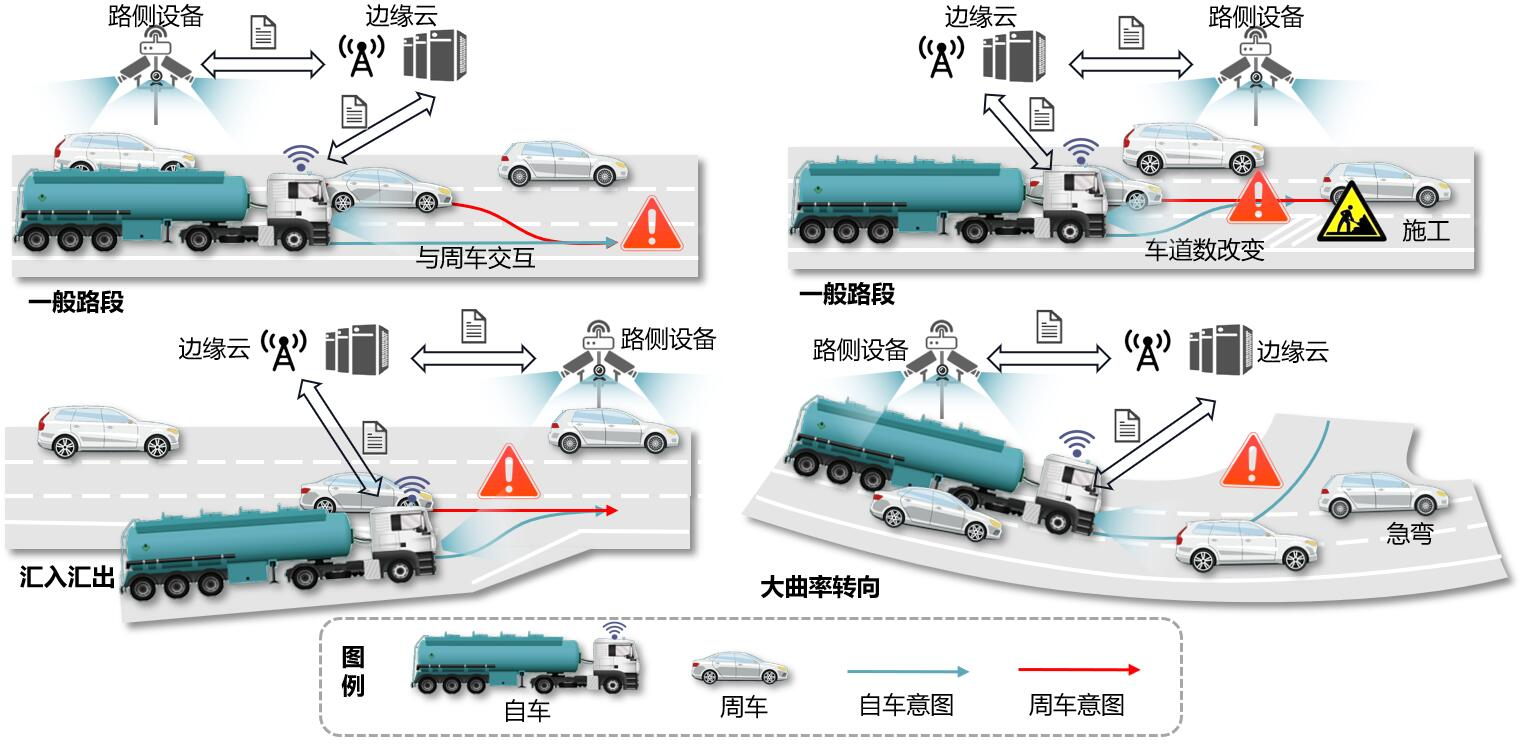
\includegraphics[width=0.9\linewidth]{fig/chap1/use_case.jpg}
      % \caption*{图片注释解释说明}
      \caption{研究对象示意图}
      \label{fig:use_case}
    \end{figure} 

    本研究主要针对自动驾驶半挂式液罐车，兼顾可实现转向控制的人工驾驶半挂式液罐车，基于如下考虑：首先，液罐车分为整体式与半挂式，其中半挂式占绝大多数，且载重量大、质心高、控制难度高，相较于整体式更为危险，所以对半挂式液罐车的防侧翻研究将更有实际意义；其次，由于液罐车运输的货物运量大、危险性高、驾驶强度大、对驾驶员技术要求高，本研究认为其未来将被技术成熟、遵守法规、节省驾驶员成本的自动驾驶液罐车取代。故选取自动驾驶半挂式液罐车作为主要研究对象，假设其具有基本的环境感知（对一定范围内的道路结构、周车的感知能力）、决策与规划、闭环控制能力；兼顾转向助力系统支持实现转向控制驾驶辅助功能的人工驾驶半挂液罐车，作为快速推广算法、保障当下危化品液体运输安全的手段。

    本文的研究目标为充分发挥高等级公路云控系统的广域感知和高并行算力优势，将车云协同预测性防侧翻决策与规划与更精确的车端防侧翻控制相结合，在不降低通行效率与经济性的情况下进一步提高液罐车行驶过程的侧翻稳定性并减少陷入危险情况的概率。

  \subsection{研究现状总结及存在的问题}

    通过分析国内外研究现状可知，车云协同下的液罐车防侧翻行驶规划与控制是当前国内外交通与车辆学科的前沿领域，而相关研究方法还相对初步，主要存在以下几方面不足：

    （1）针对车液耦合动力学建模描述问题，现有研究一般采用单摆模型描述液体晃动，但建立在二维平面上的描述虽然能反映液体在车辆侧倾和侧向移动自由度的主要动态，但未考虑不可避免的横纵向耦合流动，尤其是纵向流动对横向动力学的影响。此外，现有研究还忽略了对车辆行驶有重要影响的其他模态，如液体晃动对横摆模态的影响，也尚未考虑不同道路横纵向坡度情况下的稳态液体动力学差异。

    （2）针对车辆防侧翻控制问题，一方面，现有研究在未侧翻模态尚未考虑反应更多关键模态液体晃动模型的加入以及将控制手段结合防侧翻规划，且限于安全问题尚未有进行液罐车防侧翻的实车与模型验证。虽有很多关于流体力学相似性的基础性研究，但同样鲜有关于车辆和液体动力何时同时满足的研究。另一方面，针对危险工况下可能出现的半侧翻模态，目前缺乏对于此状态可控性、动力学特性以及控制方法的研究。

    （3）针对车云协同预测性决策与规划问题，现有研究对于非受控的周车的长时域行为预测过于简单，鲜有考虑这些车辆参数与意图的不确定性，或只考虑了短时域的不确定性进行决策，建模方法只能反映出有限的可能性，得出的结论较为理想，未能充分发挥车云协同的感知与算力优势。且目前尚未有针对液罐车的防侧翻运动规划研究，而现有车端运动规划方法在危险情况下不考虑液体晃动，难以直接应用在液罐车上。

    （4）对于车云协同液罐车防侧翻体系建设而言，目前该体系尚未形成，各类研究重心较为分散，并未有从体系工程角度从车辆控制、规划与车云协同体系的角度共同出发，以整体为优化目标解决问题的尝试。

  \subsection{总体研究方案}

    本研究基于云控系统，提出了车云协同液罐车防侧翻行驶规划与控制架构，旨在通过云控系统的全局感知，使得液罐车可以精确掌握周围的道路结构、临时施工、周车状态与意图等动静态交通信息（外因、人因）；通过云控系统的强大并行算力，可以考虑目标液罐车的侧翻特性，结合周围车辆状态与意图信息，进行预测性决策与防侧翻轨迹规划（内因、人因）；通过车端的短时域规划与双模态轨迹跟踪防侧翻控制结合横纵向耦合液体晃动模型，提供紧急时刻的兜底保障（内因、人因），以提高系统可靠性与可应用性，对危化品公路运输安全保障的强化具有十分重要的意义。为实现上述研究目标，本文将围绕车云协同液罐车防侧翻行驶规划与控制架构、车云协同预测性决策与防侧翻规划、车端态防侧翻控制与缩比液罐车实验验证等方面开展研究，本研究的总体研究方案如图~\ref{fig:thesis_archi}所示



    \subsubsection*{(1)车云协同液罐车防侧翻行驶架构}

    首先进行本场景下的场景任务体系架构构建：从信息物理体系的视角对研究对象进行分析，解析体系组成，并结合IVCPS体系架构框架的指导采用So-MBSoSE方法构建本场景下的体系架构，形成体系级防侧翻解决方案。最后，采用架构在环逻辑仿真对所构建的架构进行验证，以在验证完成的架构基础上实现车云协同决策与规划算法及车端控制算法。

    \begin{figure}
      \centering
      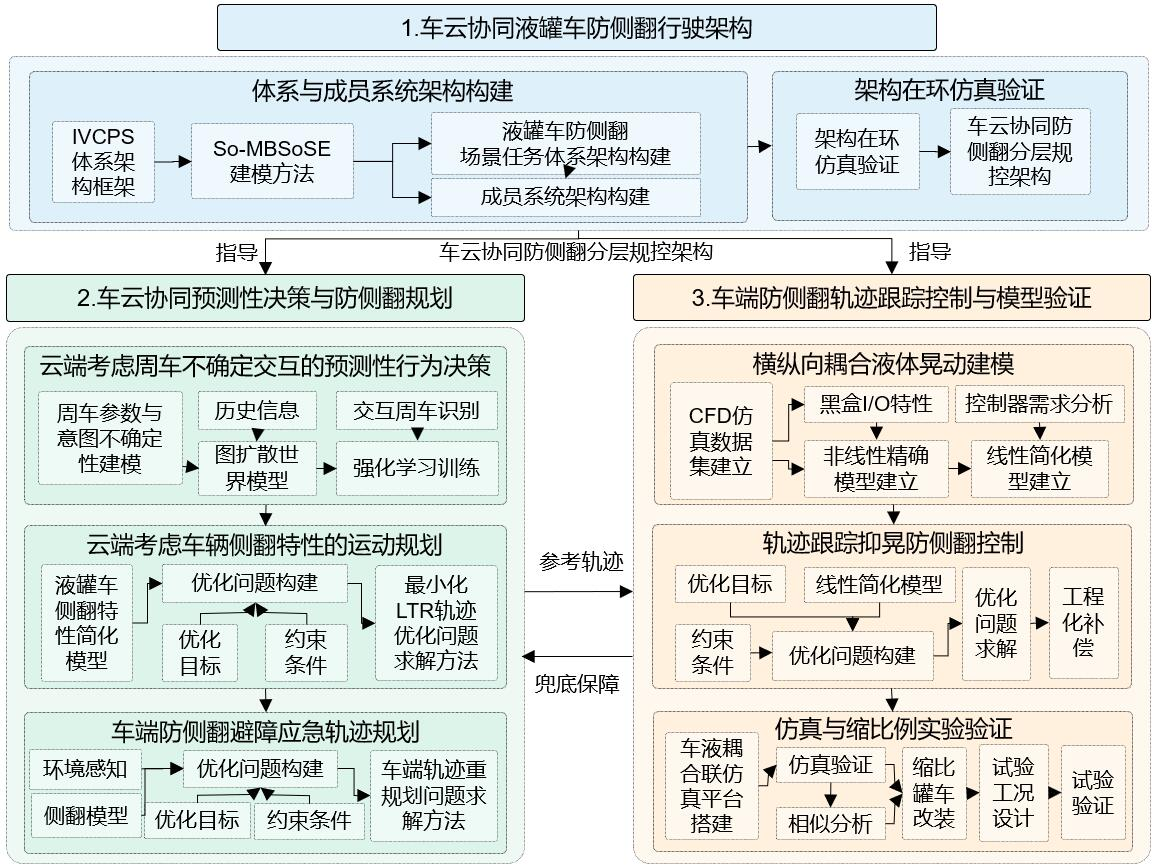
\includegraphics[width=1.0\linewidth]{fig/chap1/architecture.jpg}
      % \caption*{图片注释解释说明}
      \caption{本文研究框架}
      \label{fig:thesis_archi}
    \end{figure} 

    \subsubsection*{(2)车云协同预测性决策与防侧翻规划}

    在上述车云协同架构指导下，为从源头防止液罐车陷入危险工况，需要结合云端的广域感知和强大并行算力与车端对应急事件的实时响应能力进行车云协同预测性决策与防侧翻轨迹规划。首先，在云端进行低频率考虑周车不确定性交互的预测性行为决策：建立包含周车参数和意图不确定性的图扩散预测世界模型，并根据云端的周车历史信息与自车意图在世界模型进行推演实现智能体训练，考虑最小化20s长时域累计风险且保证行驶效率与舒适性的预测性决策。其次，根据行为决策结果进行考虑车辆简化侧翻特性的运动规划。以LTR为侧翻状态指标，找到该行为决策下使得$‖LTR‖_∞$最小化的换道轨迹，将该轨迹下发车端。最后，在车端建立简化侧翻模型考虑周车实时意图与最可能及最危险两种情况下的高频率的防侧翻避障应急轨迹规划。车辆根据感知结果自主判断云端建议是否可执行，若不可执行，则启动车端应急轨迹规划生成一条考虑侧翻特性的紧急避障轨迹用于跟踪。

    \subsubsection*{(3)车端防侧翻轨迹跟踪控制与模型试验}

    在上述车云协同架构指导下，为保证基本稳定能力，研究三聚焦于车液耦合动力学建模与防侧翻控制。首先进行横纵向耦合液体晃动建模：建立标准工况下的3D液体CFD数据集，并分析其黑盒输入输出特性，在此基础上建立非线性精确动力学模型用于云端构建的快速算法仿真验证平台，以及车端进行液体状态的推演。最后，分析车端控制器对于简化模型的需求，线性化对控制效果影响最大的模态，并将其与半挂车动力学模型结合，建立线性化半挂液罐车模型及其随运行工况的重线性化机制。其次，针对未侧翻模态进行轨迹跟踪抑晃防侧翻控制多目标最优控制问题，并在车端求解。此外，还考虑通过控制器嵌套的方式将算法用于辅助人工驾驶。最后，通过通过构建车液耦合仿真平台和缩比液罐车实验平台作为上述方法验证的手段。编写代码以MATLAB/Simulink为桥梁实现流体力学仿真软件StarCCM+和车辆动力学仿真软件TruckSim的联合仿真；其次构建云控缩比液罐车实验平台，包括液罐车改装、通信链路构建等，并进行实验相似性原则分析，以确保车辆侧翻动力学和流体力学同时满足相似性。最后，依据相似性原则进行试验工况设计并开展试验验证工作。

  \subsection{本文创新点与主要贡献}

    围绕“车云协同液罐车防侧翻行驶规划与控制”这一核心目标，本文主要创新点与贡献概括如下：
    \begin{itemize}
      \item \emph{体系架构层}：面向云控系统下液罐车防侧翻场景，基于IVCPS框架并采用So-MBSoSE方法构建可实现、可验证的场景任务体系架构，并通过架构在环进行一致性验证，为算法落地提供系统边界与接口约束。
      \item \emph{云端预测性决策层}：面向低渗透率交通流中周车参数与意图不确定性，构建图扩散交互式预测世界模型并用于长时域风险累积最小化的预测性决策学习，充分发挥云端广域感知与并行算力优势。
      \item \emph{防侧翻规划层}：以LTR等侧翻指标刻画车辆侧倾风险，形成与云端行为决策一致的防侧翻换道轨迹生成与下发机制，并在车端增加可执行性判别与应急兜底规划以提升闭环可靠性。
      \item \emph{车液耦合建模与控制层}：面向液体晃动的横纵向耦合特征，建立能够服务于控制设计与在线重线性化的车液耦合模型，并提出兼顾轨迹跟踪与抑晃防侧翻的多目标最优控制框架。
      \item \emph{验证层}：构建车液耦合联合仿真与缩比实验平台，结合相似性原则进行工况设计，对车云协同规划与车端控制方法的有效性与可实现性进行验证。
    \end{itemize}

  \subsection{论文结构安排}
    
    本文共分为五章，各章内容安排如下：
    \begin{itemize}
      \item 第1章：引言。阐述研究背景与意义，综述国内外研究现状，明确研究对象、关键问题与总体技术路线。
      \item 第2章：车云协同防侧翻场景任务体系架构设计。基于体系架构方法构建并验证车云协同液罐车防侧翻行驶分层决控架构。
      \item 第3章：车云协同预测性决策与防侧翻规划。构建图扩散交互预测模型与强化学习长时域决策方法，并给出车端应急轨迹规划与仿真验证。
      \item 第4章：车端防侧翻轨迹跟踪控制与模型试验。开展横纵向耦合液体晃动建模、抑晃防侧翻控制设计，并完成联合仿真与缩比试验验证。
      \item 第5章：总结与展望。总结全文研究工作与主要贡献，讨论不足并展望未来研究方向。
    \end{itemize}

